% The Adolescent Scar of Early-Life Disaster — tables and instrument appendix
% Estándar de formato: WP de la Jornada (AER-style). Fragmentos generados por
% scripts/15_paper_estimaciones.py y scripts/16_apendice_instrumentos.py.
% Compilar: pdflatex -interaction=nonstopmode tablas.tex (x2)
\documentclass[12pt]{article}

\usepackage[utf8]{inputenc}
\usepackage[T1]{fontenc}
\usepackage{mathptmx}
\usepackage{amssymb}
\usepackage[margin=1in]{geometry}
\usepackage{booktabs,threeparttable}
\usepackage{graphicx}
\usepackage[figuresright]{rotating}
\usepackage{float}
\usepackage{amsmath}
\usepackage{setspace}
\usepackage{caption}
\usepackage[table]{xcolor}
\usepackage[hidelinks]{hyperref}
\usepackage{etoolbox}
\usepackage{relsize}

% estout imprime los asteriscos con \sym, que no define ningun paquete cargado.
\providecommand{\sym}[1]{\ensuremath{^{#1}}}

\graphicspath{{figures/}}

%---- Tablas al estilo AER: TABLE 1—TÍTULO, versalitas, sin dos puntos -------
\DeclareCaptionLabelSeparator{emdash}{---}
% Captions de tabla al estilo de Gillmore (2026, EER): "Table N" en negrita,
% salto de linea y frase descriptiva en redonda, alineadas a la izquierda.
\captionsetup[table]{labelsep=newline,labelfont=bf,textfont=normalfont,
 justification=raggedright,singlelinecheck=false,skip=4pt}
\captionsetup[figure]{labelsep=period,justification=centering,
 singlelinecheck=false,skip=6pt}

% Estilo unico de tabla: se aplica a todas, y los .tex ya no lo declaran.
\newcommand{\tabstyle}{\singlespacing\small\setlength{\tabcolsep}{5pt}\renewcommand{\arraystretch}{1.05}}
\AtBeginEnvironment{table}{\tabstyle}
\AtBeginEnvironment{sidewaystable}{\tabstyle}
\AtBeginEnvironment{figure}{\singlespacing}
\newcommand{\flushhead}{}

% Notas: un escalon por debajo del cuerpo, con el ancho de la tabla.
\newenvironment{wpnotes}{\par\vspace{6pt}\begin{tablenotes}[flushleft]\relsize{-1}\setlength{\parindent}{0pt}\item[]}{\end{tablenotes}}
\newenvironment{fignotes}[1][0.9\textwidth]{\par\vspace{6pt}\begin{minipage}{#1}\footnotesize\setlength{\parindent}{0pt}}{\end{minipage}}
\newcommand{\panel}[2]{\multicolumn{#1}{@{}l}{\textit{#2}}\\}

%---- Frases unicas, reutilizadas por las notas de todas las tablas ----------
\newcommand{\starnote}{*** Significant at the 1 percent level. ** Significant at the 5 percent level. * Significant at the 10 percent level.}
\newcommand{\bindef}{Exposure-age groups give the child's age when the earthquake struck, defined in months of age as 0--11 (before age 1, the omitted group), 12--23 (age 1), 24--35 (age 2) and 36--59 (ages 3--4). Each coefficient compares the gap between the age group in the row and the omitted group in affected municipalities with the same gap in unaffected municipalities.}
\newcommand{\zonedef}{The affected zone comprises the six regions where the official intensity study records destructive shaking (V, VI, VII, VIII, IX and Metropolitan; Astroza et al.\ 2010).}
\newcommand{\specdef}{Column 1 includes exposure-age, municipality-of-selection and birth-cohort fixed effects; column 2 adds pre-earthquake controls (sex, age in months, and the 2010 household baseline: mother's education and age, household size, rurality); column 3 adds 2012 controls (number of children of the mother, family history of mental illness), with missing-value indicators; column 4 estimates column 3 without the Metropolitan Region. Estimates use the 2024 sampling weights.}
\newcommand{\phqdef}{The PHQ-4 is a four-item screener (two depression, two anxiety items) answered by the adolescent in private, scored 0--12 and standardized within age in years; a positive PHQ-2 (GAD-2) screen is a depression (anxiety) subscore of three or more, and coefficients for these outcomes are probabilities.}
\newcommand{\cbcldef}{The CBCL internalizing score is reported by the main caregiver, in T units, standardized within age.}
\newcommand{\clusternote}{Standard errors clustered by municipality of selection in parentheses.}

\doublespacing

\usepackage{placeins}
\begin{document}

\begin{titlepage}
\centering
\vspace*{2cm}
{\Large\bfseries The Adolescent Scar of Early-Life Disaster\par}
\vspace{1.5cm}
{\large José Elías Durán Roa\par}
\vspace{1cm}
{\large \today\par}
\vspace{1cm}
{\normalsize Tables and instrument appendix --- draft for discussion\par}
\end{titlepage}

\setcounter{page}{1}

\begin{center}
{\scshape Overview}
\end{center}

The 27 February 2010 earthquake, of magnitude 8.8, struck a large part of
Chile in the middle of the night. Fourteen years later the ELPI, Chile's
early-childhood panel, returned to children who were between six months
and four years old that day and, for the first time, asked the adolescents
themselves about their mental health. This paper asks whether a disaster
lived through in early childhood leaves a mark on mental health in
adolescence, and whether that mark depends on the age at which the disaster
struck. The question matters because early childhood is when the systems
that regulate stress and emotion are built, and a child cannot choose when
a disaster arrives. If the same shock leaves a deeper mark at some ages than
at others, the age at exposure becomes a dimension of vulnerability in its
own right. The children who lived the shock at the most sensitive ages are
then those who may need attention years later, long after the
reconstruction has ended.

There are two routes through which an earthquake may reach the mental
health of a young child. The first is direct. The child lives the shaking
and the months of aftershocks that follow, and from around age three
children understand danger and can remember it. Preschool children develop
post-traumatic symptoms after disasters (Scheeringa and Zeanah 2008). The
second route runs through the family, which absorbs the shock and passes it
on. Lost income and damaged homes raise parental stress and harshen
parenting, the mechanism of the family stress model (Conger and Donnellan
2007); maternal depression is among the strongest predictors of anxiety and
depression in children (Goodman et al.\ 2011). Family conflict and
maltreatment rise after disasters (Keenan et al.\ 2004), and routines, child
care and health services are disrupted for months. For a breastfed infant
the mother's body is itself part of the environment, since maternal
cortisol reaches the infant through the milk (Glynn et al.\ 2007; Hinde et
al.\ 2015). Both routes converge on what the child is building at that age,
the systems that regulate stress and emotion (Gunnar and Quevedo 2007).

These early effects may last into adolescence for several reasons. Systems
under construction are the most malleable, so a shock that arrives while
they form can shift their set point rather than only their state at the
time (Knudsen 2004; Cunha and Heckman 2007). Stress also affects each brain
region most strongly while that region is developing (Lupien et al.\ 2009).
A stress system calibrated in adversity reacts more strongly to later
stressors (Hammen et al.\ 2000), and adolescence brings many of them.
Moreover, anxiety and depression typically emerge in adolescence, when the
gap between girls and boys opens (Salk et al.\ 2017), so an early
vulnerability may remain silent during childhood and surface only after
puberty. Finally, the exposure itself may outlast the event if the mother's
mental health or the family's finances remain worse for years. In
economics, Persson and Rossin-Slater (2018) show that prenatal stress caused
by the death of a relative increases the use of mental-health medication in
adulthood, and Almond et al.\ (2018) review a large literature on the long
reach of early-life circumstances.

In this paper we compare adolescents who lived through the earthquake at
different ages within the same municipality. We then compare these age gaps
between the municipalities where the earthquake caused destructive shaking
and those where it did not. This design has a feature that shapes the whole
interpretation. Shocks that hit the household as a whole (e.g., lost income,
a damaged home or a distressed mother) reach an infant and a four-year-old
alike, and they cancel out when we compare exposure ages. What the design
detects is whether the same shock weighed differently depending on the
stage of development at which it arrived. By construction, the paper
therefore studies when the earthquake left a mark rather than how large the
average mark is.\footnote{Municipality fixed effects absorb the difference
between affected and unaffected municipalities, so the design identifies
how outcomes vary across exposure ages, not their level.
Table~\ref{tab:longrun} recovers levels for the vocabulary and
caregiver-reported scores, which the ELPI also measured in 2017 for
children conceived after the earthquake. The PHQ-4 was answered only by
adolescents born between 2006 and 2009, all of whom lived through the
earthquake.} We use the four waves of the ELPI, collected in 2010, 2012,
2017 and 2024, which follow 10,003 adolescents born between 2006 and 2009
from ages 0--4 in 2010 to ages 15--18 in 2024. Mental health is measured
with the PHQ-4, a screener of four questions on low mood, loss of interest,
nervousness and worry that the adolescents answer in private.\footnote{The
PHQ-4 adds four items scored from 0 to 3, so the scale runs from 0 to 12. A
subscore of three or more on its two depression items, the PHQ-2, or on its
two anxiety items, the GAD-2, is the standard positive screen (Kroenke et
al.\ 2009). We standardize the index within age in years, and Appendix
Table~\ref{tab:a_mh} reproduces every question.}

The earthquake left a mark whose depth depends on the age at which it
struck. In the full sample, adolescents exposed at age two report fewer
symptoms at ages 15--18 than adolescents exposed before age one. Their
PHQ-4 is 0.39 points lower on its 0-to-12 scale, or 0.147 standard
deviations, statistically significant at the 5 percent level (column 3 of
Panel A in Table~\ref{tab:main}). The magnitude is moderate. The index
averages 4.31 points in the sample, so the gap corresponds to 9 percent of the mean and to about a third
of the distance between girls and boys. Adolescents exposed at ages three
and four also report more symptoms than those exposed at age two, by 0.103
standard deviations, statistically significant at the 10 percent level
(column 1 of Table~\ref{tab:specific}). The age profile has the shape of a
U, with its trough at age two (Figure~\ref{fig:ushape}). The anxiety half
of the index moves the most, since the probability of a positive GAD-2
screen falls by 7.3 percentage points at age two relative to a base of 27.3
percent.

The profile belongs to girls. Among girls, exposure at age two lowers the
PHQ-4 by 0.300 standard deviations relative to exposure in infancy,
statistically significant at the 1 percent level. The anxiety screen falls
by 13.7 percentage points and the depression screen by 11.7. Girls exposed
at ages three and four report 0.182 standard deviations more symptoms than
girls exposed at age two, statistically significant at the 5 percent level
(column 4 of Table~\ref{tab:specific}). Among boys every estimate is close
to zero and statistically insignificant (Table~\ref{tab:het}). Weighting
both groups by their shares of the sample, girls account for 95 percent of
the age-two coefficient and for 81 percent of the gap between exposure at
ages three and four and exposure at age two. The caregivers of the same
adolescents report no gradient at any age, neither in 2024 nor in the
change since 2017 (Table~\ref{tab:caregiver}). This is consistent with
symptoms that adolescents feel and adults do not observe, and with a
vulnerability that remained silent during childhood.

The adolescents exposed at age two are not simply a luckier cohort. If the
cohort exposed at age two in the affected municipalities were better off in
every respect, it would also have a better vocabulary, and it does not. In
the 2024 vocabulary test, adolescents exposed at age two score 0.119
standard deviations below those exposed at ages three and four,
statistically significant at the 5 percent level. The age profile of
mental health differs significantly from the age profile of vocabulary,
both in the full sample and among girls (columns 3 and 6 of
Table~\ref{tab:specific}). The vocabulary result fits what Gillmore (2026)
documents after the same earthquake. The vocabulary loss he measures at
ages 7--11, of 0.17 standard deviations, is still there at ages 15--18, at
0.24, while the caregiver-reported behavior problems he finds at ages
7--11 are gone (Table~\ref{tab:longrun}). Age two falls in the period in
which children's vocabulary grows fastest, so the same shock may have
reached language rather than mental health in that cohort. Our data are
consistent with this interpretation but cannot test it directly.

Among the infants, the mark concentrates in those who were still breastfed
on the day of the earthquake. According to their mothers' report in 2012,
62 percent of the children exposed at 6--11 months were breastfed at the
time. Among them, living in an affected municipality raises the PHQ-4 at
ages 15--18 by 0.364 standard deviations more than among the infants who
were not breastfed, statistically significant at the 1 percent level
(column 1 of Panel A in Table~\ref{tab:breast}). In the unaffected
municipalities the breastfed infants report fewer symptoms as
adolescents, and in the affected municipalities this advantage
disappears. Among girls the interaction reaches 0.549 standard
deviations. Among the children exposed
at age one the same interaction is close to zero.\footnote{Among the
children exposed at age two the interaction is negative and significant at
the 10 percent level (column 5 of Panel A in Table~\ref{tab:breast}), but
only 14 percent of them were still breastfed, a highly selected group.} The
breastfed and non-breastfed infants of the affected municipalities were not
different before the earthquake, since the interaction is small and
statistically insignificant for birth weight, birth length, gestation, and
the mother's schooling and age (Panel B). The pattern is consistent with
maternal stress reaching the infant through breastfeeding (Glynn et al.\
2007; Hinde et al.\ 2015), a potential physiological channel. However, the
data do not measure cortisol and cannot separate the stress that passed
through the milk from the disruption of breastfeeding itself.

The household channels that reach children of every age do not explain the
profile, as the design predicts. Neither in 2012 nor in 2017 did the
children exposed as infants witness more fights at home or receive harsher
discipline than the children exposed at age two. If anything, the latter
were yelled at more often in 2017 (Table~\ref{tab:home}). The adolescents
exposed as infants do report more fights at home in 2024, when their
symptoms are already present. Controlling for those reports barely moves
the gap among girls, from 0.307 to 0.288 standard deviations in the sample
with both measures.

The excess of symptoms among girls exposed at ages three and four has no
demonstrated channel. The literature on early memory offers one, since from
around age three children begin to form memories of distressing events that
can last (Terr 1988; Bauer 2007; Alberini and Travaglia 2017). The trough at
age two would then fall in the window of infantile amnesia, after the
infant's dependence on the mother's body and before the child can
understand and remember what happened. Our data do not confirm this
interpretation, and we leave it as an open question.\footnote{Four tests
point against a simple version of this hypothesis. In the 2010 wave,
collected between one and nine months after the earthquake, girls exposed
at ages three and four show more emotional reactivity than girls exposed at
age two in their caregivers' CBCL, but not more internalizing problems
overall. Their gap in 2024 does not vary with the damage the earthquake
caused to the dwelling, and it is larger when the mother reported distress
after the earthquake, but not significantly so. A comparison around the
school-entry cutoff of March 2010 produces a jump that vanishes when the
window narrows. The cohort exposed at age two in the affected
municipalities was also born after slightly shorter gestations, and adding
the birth outcomes as controls leaves every estimate unchanged.}

Our study contributes to three strands of literature. First, a large
literature documents the long reach of early-life circumstances (Almond et
al.\ 2018), including the effect of stress around birth on adult mental
health (Persson and Rossin-Slater 2018). We show that within early
childhood the timing of a shock shapes which outcome it reaches, since
mental health and vocabulary follow opposite age profiles. Second, a
literature on disasters and children documents effects on birth outcomes
and on child development (Torche 2011; Gillmore 2026). We follow the same
children for fourteen years and measure mental health with the adolescents'
own reports, which the caregiver reports used in this literature miss.
Third, the developmental literature on sensitive periods relies mostly on
correlational studies of adversity (Lupien et al.\ 2009). The earthquake
provides a common shock whose timing relative to each child's birth is as
good as random, and the breastfeeding result points to a potential
physiological channel. The next section presents the empirical strategy,
and the tables follow.

\begin{center}
{\scshape Empirical Strategy}
\end{center}

Every adolescent of the 2024 wave lived through the earthquake as a child,
and identification rests on the two things that vary across them, how hard
their municipality was shaken and how old they were when it struck, with
age grouped as 0--11 months (the omitted group), 12--23, 24--35 and
36--59. We compare the outcome gap between two exposure ages within the
municipalities the earthquake hit against the same gap within the
municipalities it did not hit, so municipality fixed effects keep every
comparison local and birth-cohort fixed effects absorb everything a cohort
shares, including its age at the survey. All tables estimate versions of
\begin{equation}
Y_{imc} \;=\; \alpha \;+\; \sum_{a}\beta_a\,\bigl(\text{Bin}_{ai}\times D_m\bigr)
\;+\; \sum_{a}\gamma_a\,\text{Bin}_{ai} \;+\; \psi_m \;+\; \theta_c
\;+\; X_i'\delta \;+\; \varepsilon_{imc},
\end{equation}
where $Y_{imc}$ is the outcome of adolescent $i$ of birth cohort $c$ in
municipality $m$; $\text{Bin}_{ai}$ are the exposure-age groups; $D_m$
equals one in the six regions where the official intensity study records
destructive shaking (V to IX and the Metropolitan Region; Astroza et al.\
2010); $\psi_m$ and $\theta_c$ are municipality-of-selection and
birth-cohort fixed effects; $X_i$ are household controls; and
$\varepsilon_{imc}$ is the error term. The coefficients of interest are
the $\beta_a$, the effect of having lived the earthquake in an affected
municipality at age $a$ relative to the children exposed before age one.
The main effects $\gamma_a$ absorb the outcome differences across
exposure-age groups that are common to affected and unaffected
municipalities, differences that exist mechanically because a child who
was older at the earthquake is also older at the 2024 interview, and
$\beta_a$ is therefore identified only from how that age profile differs
between the two zones.
Standard errors are clustered by municipality of selection, and estimates use
the 2024 sampling weights.

\clearpage

% ---- begin paper/tables/t1_descriptivos.tex
\begin{table}[htbp]\centering
\begin{minipage}{360pt}
\caption{Descriptive statistics.}
\label{tab:sample}
{\small
\begin{tabular*}{360pt}{@{}l@{\extracolsep{\fill}}lll@{}}
\toprule
 & (1) & (2) & (3) \\
 & Non-Earthquake & Earthquake & Difference \\
\midrule
Girl & 0.489 & 0.489 & $-$0.000 \\
 & (0.500) & (0.500) & (0.011) \\
Age at the earthquake (months) & 26.930 & 27.098 & 0.169 \\
 & (12.710) & (12.614) & (0.254) \\
Mother's age (2010) & 28.980 & 29.676 & 0.695\sym{***} \\
 & (7.066) & (7.116) & (0.196) \\
Mother's schooling (2010) & 10.312 & 10.311 & $-$0.002 \\
 & (3.182) & (3.180) & (0.211) \\
HH size (2010) & 4.865 & 4.948 & 0.083 \\
 & (1.641) & (1.686) & (0.074) \\
Rural household (2010) & 0.080 & 0.094 & 0.014 \\
 & (0.271) & (0.292) & (0.035) \\
Children of the mother (2012) & 2.165 & 2.155 & $-$0.010 \\
 & (1.072) & (1.075) & (0.029) \\
Prior mental health, mother (2012) & 0.091 & 0.125 & 0.034\sym{***} \\
 & (0.288) & (0.331) & (0.012) \\
Prior mental health, father (2012) & 0.023 & 0.027 & 0.004 \\
 & (0.150) & (0.161) & (0.004) \\
Prior mental health, relative (2012) & 0.123 & 0.152 & 0.029\sym{*} \\
 & (0.328) & (0.359) & (0.017) \\
\addlinespace[6pt]
Observations & 2,349 & 7,654 & 10,003 \\
\bottomrule
\end{tabular*}\par}
\vspace{4pt}
{\footnotesize
\textit{Notes}: ELPI uses sampling weight at national level. The sample are the 10,003 adolescents of the 2024 wave, born January 2006--August 2009, aged 6 to 49 months on the day of the earthquake and 15 to 18 at the 2024 interview. Sex and ages are fixed at birth and the 2010 rows come from the pre-earthquake baseline; the 2012 rows are the family size and the lifetime conditions reported in the 2012 wave, the controls of the main specification, and are missing for adolescents without that interview. Mental health rows mark a reported diagnosis of depression, anxiety, bipolar disorder, schizophrenia, a personality disorder or an autism spectrum disorder. Earthquake municipalities are those of the six regions where the official intensity study records destructive shaking (V, VI, VII, VIII, IX and Metropolitan; Astroza et al. 2010). Column 3 is the difference from a regression on the earthquake indicator; standard errors clustered at the municipality of selection appear in parentheses---number of clusters: 116. * p $<$ 0.1, ** p $<$ 0.05, *** p $<$ 0.01.
\par}
\end{minipage}
\end{table}
% ---- end paper/tables/t1_descriptivos.tex

% ---- begin paper/tables/t2_largo_plazo.tex
\begin{table}[htbp]\centering
\begin{minipage}{460pt}
\caption{The impact of the earthquake on cognitive and non-cognitive development in the medium- and long-term.}
\label{tab:longrun}
{\small
\begin{tabular*}{460pt}{@{}l@{\extracolsep{\fill}}llll@{}}
\toprule
 & \multicolumn{2}{@{}l}{Medium-term effect (Gillmore)} & \multicolumn{2}{@{}l}{Long-term effect} \\
 & \multicolumn{2}{@{}l}{2017 wave} & \multicolumn{2}{@{}l}{2024 wave} \\
\cmidrule(r){2-3}\cmidrule(l){4-5}
 & (1) & (2) & (3) & (4) \\
\midrule
\textbf{\textit{Panel A: Peabody}} & & & & \\
Affected$\times$Earthquake & $-$0.174\sym{**} & $-$0.280\sym{***} & $-$0.240\sym{**} & $-$0.412\sym{**} \\
 & (0.0686) & (0.0866) & (0.104) & (0.180) \\
\addlinespace[9pt]
Observations & 14,069 & 14,069 & 13,779 & 13,779 \\
\addlinespace[9pt]
\textbf{\textit{Panel B: CBCL2}} & & & & \\
Affected$\times$Earthquake & $-$0.129\sym{*} & $-$0.220\sym{**} & 0.084 & $-$0.066 \\
 & (0.0763) & (0.105) & (0.0884) & (0.125) \\
\addlinespace[9pt]
Observations & 11,568 & 11,568 & 11,038 & 11,038 \\
\addlinespace[9pt]
Municipality FE & \checkmark & \checkmark & \checkmark & \checkmark \\
Birth Cohort FE & \checkmark & \checkmark & \checkmark & \checkmark \\
Child-Mother-HH control & \checkmark & \checkmark & \checkmark & \checkmark \\
Municipality linear trends & $\times$ & \checkmark & $\times$ & \checkmark \\
\bottomrule
\end{tabular*}\par}
\vspace{4pt}
{\footnotesize
\textit{Notes}: Each column represents a separate regression. The dependent variable is the test score measured in standard deviations. Peabody is the Peabody Test Score and CBCL is the Child Behavior Check List measure, oriented so that higher means fewer problems. Columns 1 and 2 reproduce Columns 3 and 4 of Table 3 in Gillmore (2026): children exposed between in utero and age four, with scores measured seven years later, at ages 7--11; our replication of his Column 3 on the public ELPI files gives $-$0.160 for Peabody and $-$0.103 for CBCL2. Columns 3 and 4 estimate the same two specifications on the 2024 wave: the same exposed children measured fourteen years later, at ages 15--18, against the comparison group conceived after the earthquake and measured in 2017; pooling the two waves adds survey-wave fixed effects, as in Gillmore's short-term table. Standard errors clustered at the municipal level appear in parentheses---number of clusters: 145 in Columns 1 and 2 and 116 in Columns 3 and 4. The estimates use sampling weights. Child/Mother/HH characteristics include gender, age at the moment of the test (in months), birth order, mothers' age and schooling, father present, number of household members, prior mental health condition for mother, father and relative. * p $<$ 0.1, ** p $<$ 0.05, *** p $<$ 0.01.
\par}
\end{minipage}
\end{table}
% ---- end paper/tables/t2_largo_plazo.tex

\FloatBarrier

\begin{figure}[htbp]\centering
  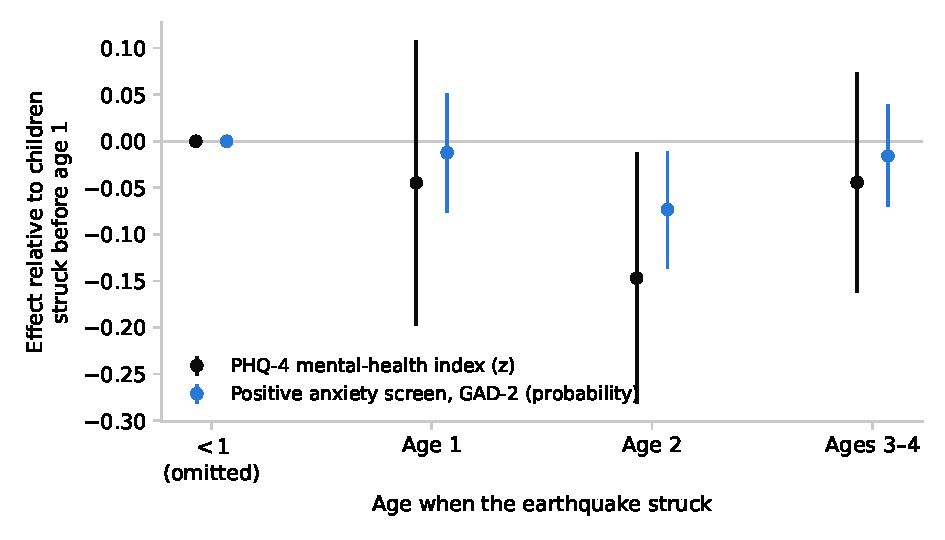
\includegraphics[width=0.9\textwidth]{f1_gradiente_u.pdf}
  \caption{Estimates by Age at Exposure}
  \label{fig:ushape}
  \begin{fignotes}[0.9\textwidth]
\textit{Notes:} Each marker is a $\beta_a$ coefficient of equation~(1) with the
controls of column 3 of Table~\ref{tab:main}, with its 95 percent confidence
interval. The reference group, drawn at zero by construction, are the children
struck at 0--11 months --- already born; children in utero during the
earthquake are not in the 2024 wave, which follows only the cohort born
2006--2009. The PHQ-4 is in standard deviations and the GAD-2 screen in
probability units. \clusternote
  \end{fignotes}
\end{figure}
\FloatBarrier

% ---- begin paper/tables/t3_main.tex
\begin{table}[htbp]\centering
\caption{Age at Exposure to the Earthquake and Self-Reported Mental Health at Ages 15--18}
\label{tab:main}
\footnotesize\renewcommand{\arraystretch}{0.95}
\begin{threeparttable}
\begin{tabular}{@{}p{182pt}*{4}{>{\centering\arraybackslash}p{64pt}}@{}}
\toprule
 & (1) & (2) & (3) & (4) \\
\midrule
\panel{5}{Panel A. Mental health: PHQ-4 index, four questions on low mood, loss of interest, nervousness and worry (0--12, z)}
Exposed at age 1 & $-$0.051 & $-$0.044 & $-$0.045 & $-$0.030 \\
 & (0.080) & (0.078) & (0.078) & (0.079) \\
\addlinespace[3pt]
Exposed at age 2 & $-$0.144\sym{**} & $-$0.153\sym{**} & $-$0.147\sym{**} & $-$0.120 \\
 & (0.072) & (0.069) & (0.069) & (0.076) \\
\addlinespace[3pt]
Exposed at ages 3--4 & $-$0.038 & $-$0.048 & $-$0.044 & $-$0.011 \\
 & (0.064) & (0.060) & (0.060) & (0.063) \\
\addlinespace
\panel{5}{Panel B. The anxiety half of the index: positive GAD-2 screen (its two anxiety questions, subscore of 3 or more)}
Exposed at age 1 & $-$0.014 & $-$0.012 & $-$0.012 & $-$0.018 \\
 & (0.032) & (0.032) & (0.033) & (0.035) \\
\addlinespace[3pt]
Exposed at age 2 & $-$0.073\sym{**} & $-$0.076\sym{**} & $-$0.073\sym{**} & $-$0.064\sym{*} \\
 & (0.032) & (0.032) & (0.032) & (0.035) \\
\addlinespace[3pt]
Exposed at ages 3--4 & $-$0.015 & $-$0.018 & $-$0.016 & $-$0.015 \\
 & (0.027) & (0.028) & (0.028) & (0.030) \\
\addlinespace
\panel{5}{Panel C. The depression half of the index: positive PHQ-2 screen (its two depression questions, subscore of 3 or more)}
Exposed at age 1 & $-$0.017 & $-$0.014 & $-$0.014 & $-$0.020 \\
 & (0.039) & (0.038) & (0.038) & (0.041) \\
\addlinespace[3pt]
Exposed at age 2 & $-$0.046 & $-$0.050 & $-$0.048 & $-$0.073 \\
 & (0.042) & (0.041) & (0.041) & (0.045) \\
\addlinespace[3pt]
Exposed at ages 3--4 & $-$0.008 & $-$0.011 & $-$0.010 & $-$0.017 \\
 & (0.032) & (0.031) & (0.031) & (0.035) \\
\midrule
Municipality fixed effects & Yes & Yes & Yes & Yes \\
Birth-cohort fixed effects & Yes & Yes & Yes & Yes \\
Pre-earthquake controls & No & Yes & Yes & Yes \\
2012 controls & No & No & Yes & Yes \\
Excludes the Metropolitan Region & No & No & No & Yes \\
Observations & 9,996 & 9,996 & 9,996 & 6,430 \\
Selection municipalities (clusters) & 116 & 116 & 116 & 67 \\
\bottomrule
\end{tabular}
\begin{wpnotes}
\textit{Notes:} Ordinary least squares estimates of equation~(1) on the adolescents of the 2024 ELPI wave; seven of the 10,003 adolescents of Table~\ref{tab:sample} drop for incomplete PHQ-4 answers. Panels B and C disaggregate the Panel A index into its two pairs of questions, expressed as clinical screens; Appendix Table~\ref{tab:a_mh} lists every question verbatim. \bindef{} \zonedef{} \specdef{} The sample is the same in every panel; column 4 has 6,430 adolescents in 67 municipalities. Demanding inference for column 3 is reported in Table~\ref{tab:robust}. \clusternote{} \starnote
\end{wpnotes}
\end{threeparttable}
\end{table}
% ---- end paper/tables/t3_main.tex


% ---- begin paper/tables/t4_informante.tex
\begin{table}[htbp]\centering
\caption{Caregiver-Reported Outcomes}
\label{tab:caregiver}
\begin{threeparttable}
\begin{tabular}{@{}p{182pt}*{4}{>{\centering\arraybackslash}p{64pt}}@{}}
\toprule
 & (1) & (2) & (3) & (4) \\
\midrule
\panel{5}{Panel A. CBCL internalizing score in 2024: caregiver checklist (T, z)}
Exposed at age 1 & $-$0.057 & $-$0.047 & $-$0.055 & $-$0.024 \\
 & (0.099) & (0.096) & (0.095) & (0.100) \\
\addlinespace[3pt]
Exposed at age 2 & $-$0.121 & $-$0.121 & $-$0.109 & $-$0.131 \\
 & (0.074) & (0.075) & (0.075) & (0.084) \\
\addlinespace[3pt]
Exposed at ages 3--4 & $-$0.086 & $-$0.084 & $-$0.077 & $-$0.069 \\
 & (0.069) & (0.068) & (0.069) & (0.074) \\
\addlinespace
\hspace{1em}Observations & 9,970 & 9,970 & 9,970 & 6,412 \\
\addlinespace
\panel{5}{Panel B. Within-child change in the same CBCL score, 2017 to 2024 (z by wave)}
Exposed at age 1 & $-$0.030 & $-$0.011 & $-$0.012 & $-$0.020 \\
 & (0.131) & (0.125) & (0.124) & (0.128) \\
\addlinespace[3pt]
Exposed at age 2 & $-$0.009 & $-$0.004 & $-$0.002 & $-$0.045 \\
 & (0.104) & (0.102) & (0.102) & (0.110) \\
\addlinespace[3pt]
Exposed at ages 3--4 & $-$0.040 & $-$0.049 & $-$0.050 & $-$0.093 \\
 & (0.109) & (0.106) & (0.106) & (0.112) \\
\addlinespace
\hspace{1em}Observations & 7,169 & 7,169 & 7,169 & 4,901 \\
\midrule
Municipality fixed effects & Yes & Yes & Yes & Yes \\
Birth-cohort fixed effects & Yes & Yes & Yes & Yes \\
Pre-earthquake controls & No & Yes & Yes & Yes \\
2012 controls & No & No & Yes & Yes \\
Excludes the Metropolitan Region & No & No & No & Yes \\
Selection municipalities (clusters) & 116 & 116 & 116 & 67 \\
\bottomrule
\end{tabular}
\begin{wpnotes}
\textit{Notes:} Same design and specifications as Table~\ref{tab:main}, with the caregiver's report of the child as the outcome. \cbcldef{} Panel B uses the change between the 2017 measurement (ages 8--12) and the 2024 measurement (ages 15--18) of the same child, each standardized within its wave and age; with two periods this is equivalent to a child fixed-effects estimate. Neither panel shows an exposure-age gradient: the scar of Table~\ref{tab:main} appears only in what adolescents report in private. \bindef{} \specdef{} \clusternote{} \starnote
\end{wpnotes}
\end{threeparttable}
\end{table}
% ---- end paper/tables/t4_informante.tex


\begin{tabular}{l rl rl c}
\toprule
 & \multicolumn{2}{c}{2 a\~nos$\times$EQ} & \multicolumn{2}{c}{Contraste 3--4$-$2} & n \\
\midrule
Mujeres & -0.300*** & (0.100) & 0.182** & (0.086) & 4,961 \\
Hombres & -0.016 & (0.098) & 0.042 & (0.086) & 5,035 \\
Madre con educ.\ media o menos (2010) & -0.107 & (0.074) & 0.071 & (0.065) & 7,755 \\
Madre con educ.\ superior (2010) & -0.201 & (0.188) & 0.182 & (0.149) & 2,053 \\
Hogar urbano 2010 & -0.139* & (0.076) & 0.129** & (0.064) & 9,005 \\
Hogar rural 2010 & -0.238 & (0.172) & -0.213 & (0.257) & 991 \\
\bottomrule
\end{tabular}


% ---- begin paper/tables/t13_especificidad.tex
\begin{table}[htbp]\centering
\begin{minipage}{460pt}
\caption{The age profile of the earthquake in mental health and in vocabulary at ages 15--18.}
\label{tab:specific}
{\small
\begin{tabular*}{460pt}{@{}l@{\extracolsep{\fill}}llllll@{}}
\toprule
 & \multicolumn{3}{@{}l}{All adolescents} & \multicolumn{3}{@{}l}{Girls} \\
\cmidrule(r){2-4}\cmidrule(l){5-7}
 & PHQ-4 & Vocabulary & Difference & PHQ-4 & Vocabulary & Difference \\
 & index & deficit & & index & deficit & \\
 & (1) & (2) & (3) & (4) & (5) & (6) \\
\midrule
Exposed at age 1 & $-$0.045 & 0.085 & $-$0.135 & $-$0.129 & 0.153 & $-$0.291\sym{*} \\
 & (0.078) & (0.089) & (0.099) & (0.124) & (0.133) & (0.152) \\
\addlinespace[3pt]
Exposed at age 2 & $-$0.147\sym{**} & 0.086 & $-$0.236\sym{**} & $-$0.300\sym{***} & 0.103 & $-$0.418\sym{**} \\
 & (0.069) & (0.079) & (0.102) & (0.100) & (0.127) & (0.165) \\
\addlinespace[3pt]
Exposed at ages 3--4 & $-$0.044 & $-$0.034 & $-$0.019 & $-$0.119 & $-$0.040 & $-$0.092 \\
 & (0.060) & (0.077) & (0.095) & (0.104) & (0.125) & (0.144) \\
\addlinespace[3pt]
Ages 3--4 $-$ age 2 & 0.103\sym{*} & $-$0.119\sym{**} & 0.218\sym{***} & 0.182\sym{**} & $-$0.143\sym{**} & 0.326\sym{***} \\
 & (0.060) & (0.053) & (0.084) & (0.086) & (0.072) & (0.122) \\
\addlinespace[6pt]
Observations & 9,996 & 9,990 & 9,986 & 4,961 & 4,956 & 4,956 \\
\addlinespace[6pt]
Municipality FE & \checkmark & \checkmark & \checkmark & \checkmark & \checkmark & \checkmark \\
Birth Cohort FE & \checkmark & \checkmark & \checkmark & \checkmark & \checkmark & \checkmark \\
Pre-earthquake controls & \checkmark & \checkmark & \checkmark & \checkmark & \checkmark & \checkmark \\
2012 controls & \checkmark & \checkmark & \checkmark & \checkmark & \checkmark & \checkmark \\
\bottomrule
\end{tabular*}\par}
\vspace{4pt}
{\footnotesize
\textit{Notes}: Each column represents a separate regression of equation~(1) with the controls of column 3 of Table~\ref{tab:main}. The PHQ-4 index is in standard deviations, so that higher values mean more symptoms. The vocabulary deficit is the 2024 TVIP score, the Spanish version of the Peabody picture vocabulary test, in standard deviations and with its sign reversed, so that higher values also mean more harm. The outcome of columns 3 and 6 is the PHQ-4 index minus the vocabulary deficit, and a coefficient different from zero in these columns means that the age profile of the earthquake differs between mental health and vocabulary. Coefficients compare each exposure-age group with the children exposed at 0--11 months, and the contrast row compares exposure at ages 3--4 with exposure at age 2. Standard errors clustered by municipality of selection appear in parentheses. The estimates use sampling weights. * p $<$ 0.1, ** p $<$ 0.05, *** p $<$ 0.01.
\par}
\end{minipage}
\end{table}
% ---- end paper/tables/t13_especificidad.tex


% ---- begin paper/tables/t14_lactancia.tex
\begin{table}[htbp]\centering
\begin{minipage}{460pt}
\caption{Breastfeeding on the day of the earthquake and mental health at ages 15--18.}
\label{tab:breast}
{\small
\begin{tabular*}{460pt}{@{}l@{\extracolsep{\fill}}lllll@{}}
\toprule
 & (1) & (2) & (3) & (4) & (5) \\
\midrule
\multicolumn{6}{@{}l}{\textbf{\textit{Panel A: Mental health at ages 15--18}}} \\
 & Infants & Infant girls & Infants & Age 1 & Age 2 \\
 & PHQ-4 & PHQ-4 & GAD-2 & PHQ-4 & PHQ-4 \\
\addlinespace[3pt]
Affected $\times$ breastfed on 27-F & 0.364\sym{***} & 0.549\sym{**} & 0.120\sym{*} & $-$0.018 & $-$0.294\sym{*} \\
 & (0.133) & (0.255) & (0.064) & (0.101) & (0.158) \\
Breastfed on 27-F & $-$0.242\sym{**} & $-$0.403\sym{*} & $-$0.063 & 0.004 & 0.254\sym{*} \\
 & (0.106) & (0.223) & (0.050) & (0.087) & (0.137) \\
\addlinespace[3pt]
Share breastfed on 27-F & 0.62 & 0.63 & 0.62 & 0.37 & 0.14 \\
Observations & 1,267 & 614 & 1,267 & 2,451 & 2,399 \\
\addlinespace[9pt]
\multicolumn{6}{@{}l}{\textbf{\textit{Panel B: Placebo, outcomes fixed before the earthquake, infants}}} \\
 & Birth & Birth & Gestation & Mother's & Mother's \\
 & weight & length & weeks & schooling & age \\
\addlinespace[3pt]
Affected $\times$ breastfed on 27-F & 0.072 & 0.100 & 0.121 & 0.119 & $-$0.024 \\
 & (0.159) & (0.152) & (0.133) & (0.126) & (0.115) \\
\addlinespace[3pt]
Observations & 1,173 & 1,167 & 1,254 & 1,255 & 1,261 \\
\bottomrule
\end{tabular*}\par}
\vspace{4pt}
{\footnotesize
\textit{Notes}: Each column represents a separate regression on one exposure-age group, infants being the children exposed at 6--11 months. Breastfed on 27-F equals one if, according to the mother in 2012, the child was still breastfed in the month of the earthquake, and the coefficient of interest is its interaction with living in an affected municipality. Panel A and columns 1 to 3 of Panel B include municipality and birth-cohort fixed effects and the controls of column 3 of Table~\ref{tab:main}; columns 4 and 5 of Panel B include only municipality fixed effects, since their outcome is itself a control. The PHQ-4 index and the Panel B outcomes are in standard deviations, and the GAD-2 screen is a probability. Among the children exposed at age 2, only 14 percent were still breastfed, a highly selected group. Standard errors clustered by municipality of selection appear in parentheses. The estimates use sampling weights. * p $<$ 0.1, ** p $<$ 0.05, *** p $<$ 0.01.
\par}
\end{minipage}
\end{table}
% ---- end paper/tables/t14_lactancia.tex


% ---- begin paper/tables/t15_hogar.tex
\begin{table}[htbp]\centering
\begin{minipage}{460pt}
\caption{Conflict and harsh discipline at home, by age at exposure to the earthquake.}
\label{tab:home}
{\small
\begin{tabular*}{460pt}{@{}l@{\extracolsep{\fill}}lllllll@{}}
\toprule
 & \multicolumn{6}{@{}l}{Mother or main caregiver} & Adolescent \\
\cmidrule(r){2-7}\cmidrule(l){8-8}
 & Fights & Yells & Threatens & Hits & Yelled, & Shook & Fights \\
 & at home & & & & insulted & or hit & at home \\
 & 2017 & 2012 & 2012 & 2012 & 2017 & 2017 & 2024 \\
 & (1) & (2) & (3) & (4) & (5) & (6) & (7) \\
\midrule
\multicolumn{8}{@{}l}{\textbf{\textit{Panel A: All adolescents}}} \\
Exposed at age 1 & $-$0.006 & 0.025 & $-$0.009 & 0.042 & 0.020 & 0.037 & $-$0.068\sym{**} \\
 & (0.027) & (0.024) & (0.038) & (0.036) & (0.040) & (0.043) & (0.027) \\
\addlinespace[3pt]
Exposed at age 2 & 0.013 & 0.006 & $-$0.021 & 0.064\sym{*} & 0.070\sym{**} & 0.002 & $-$0.099\sym{***} \\
 & (0.027) & (0.021) & (0.036) & (0.038) & (0.032) & (0.043) & (0.027) \\
\addlinespace[3pt]
Exposed at ages 3--4 & $-$0.008 & 0.014 & $-$0.058 & 0.046 & 0.038 & $-$0.001 & $-$0.078\sym{***} \\
 & (0.027) & (0.018) & (0.040) & (0.042) & (0.039) & (0.034) & (0.025) \\
\addlinespace[3pt]
Observations & 7,668 & 8,899 & 8,901 & 8,899 & 7,668 & 7,668 & 9,671 \\
\addlinespace[9pt]
\multicolumn{8}{@{}l}{\textbf{\textit{Panel B: Girls}}} \\
Exposed at age 1 & 0.004 & 0.005 & $-$0.030 & 0.007 & 0.042 & 0.070 & $-$0.065\sym{*} \\
 & (0.043) & (0.030) & (0.056) & (0.054) & (0.057) & (0.059) & (0.036) \\
\addlinespace[3pt]
Exposed at age 2 & $-$0.006 & 0.010 & $-$0.012 & 0.091 & 0.098\sym{*} & 0.086 & $-$0.092\sym{**} \\
 & (0.043) & (0.033) & (0.054) & (0.061) & (0.059) & (0.059) & (0.045) \\
\addlinespace[3pt]
Exposed at ages 3--4 & $-$0.010 & 0.016 & $-$0.056 & 0.080 & 0.041 & 0.106\sym{*} & $-$0.055 \\
 & (0.041) & (0.030) & (0.054) & (0.051) & (0.057) & (0.056) & (0.038) \\
\addlinespace[3pt]
Observations & 3,764 & 4,418 & 4,419 & 4,417 & 3,764 & 3,764 & 4,802 \\
\bottomrule
\end{tabular*}\par}
\vspace{4pt}
{\footnotesize
\textit{Notes}: Each column represents a separate regression of equation~(1) with the controls of column 3 of Table~\ref{tab:main}, and every outcome is a probability. Columns 1 and 7 equal one if the child witnessed fights or threats among household members, as reported by the main caregiver in 2017 and by the adolescent in 2024. Columns 2 to 4 come from the mother's report in 2012 of how she reacts when the child misbehaves, and equal one if she yells, threatens or hits the child at least sometimes. Columns 5 and 6 come from the main caregiver's report in 2017, and equal one if he or she yelled at, insulted or threatened the child (column 5) or shook, slapped or hit the child (column 6). In the sample of girls with both reports of fights, controlling for them moves the PHQ-4 coefficient of exposure at age 2 from $-$0.307 to $-$0.288. Standard errors clustered by municipality of selection appear in parentheses. The estimates use sampling weights. * p $<$ 0.1, ** p $<$ 0.05, *** p $<$ 0.01.
\par}
\end{minipage}
\end{table}
% ---- end paper/tables/t15_hogar.tex


\clearpage
\setcounter{table}{0}\renewcommand{\thetable}{E\arabic{table}}

% ---- begin paper/tables/b1_explora_salud.tex
\begin{table}[htbp]\centering
\begin{minipage}{460pt}
\caption{Exploratory outcomes I: mental health and well-being.}
\label{tab:explora1}
{\footnotesize\renewcommand{\arraystretch}{0.92}
\begin{tabular*}{460pt}{@{}p{200pt}@{\extracolsep{\fill}}lllll@{}}
\toprule
 & Age 1 & Age 2 & Ages 3--4 & Mean & Observations \\
 & (1) & (2) & (3) & (4) & (5) \\
\midrule
\multicolumn{6}{@{}l}{\textbf{\textit{Panel A: Mental health}}} \\
PHQ-4 symptoms (z) & $-$0.045 & $-$0.147\sym{**} & $-$0.044 & 0.000 & 9,996 \\
 & (0.078) & (0.069) & (0.060) & & \\
Positive anxiety screen, GAD-2 (0/1) & $-$0.012 & $-$0.073\sym{**} & $-$0.016 & 0.273 & 9,996 \\
 & (0.033) & (0.032) & (0.028) & & \\
Positive depression screen, PHQ-2 (0/1) & $-$0.014 & $-$0.048 & $-$0.010 & 0.346 & 9,996 \\
 & (0.038) & (0.041) & (0.031) & & \\
Internalizing problems, CBCL (z) & $-$0.026 & $-$0.071 & $-$0.044 & 0.000 & 9,552 \\
 & (0.082) & (0.076) & (0.071) & & \\
Externalizing problems, CBCL (z) & $-$0.010 & $-$0.087 & $-$0.056 & 0.000 & 9,552 \\
 & (0.079) & (0.061) & (0.061) & & \\
Attention problems, CBCL (z) & $-$0.068 & $-$0.098 & $-$0.082 & 0.000 & 9,552 \\
 & (0.088) & (0.074) & (0.061) & & \\
\addlinespace[5pt]
\multicolumn{6}{@{}l}{\textbf{\textit{Panel B: Well-being}}} \\
Resilience (z) & 0.061 & 0.141\sym{*} & 0.098 & 0.000 & 9,996 \\
 & (0.077) & (0.079) & (0.068) & & \\
Satisfaction with life in general (z) & $-$0.003 & 0.069 & 0.031 & 0.000 & 9,996 \\
 & (0.067) & (0.067) & (0.060) & & \\
Satisfaction with family life (z) & 0.086\sym{*} & 0.098\sym{*} & 0.116\sym{*} & 0.000 & 9,996 \\
 & (0.050) & (0.056) & (0.062) & & \\
Satisfaction with friends (z) & 0.048 & 0.033 & 0.030 & 0.000 & 9,996 \\
 & (0.068) & (0.063) & (0.067) & & \\
Satisfaction with school (z) & $-$0.014 & 0.032 & 0.076 & 0.000 & 9,561 \\
 & (0.067) & (0.070) & (0.073) & & \\
Satisfaction with oneself (z) & 0.055 & 0.157\sym{**} & 0.123\sym{*} & 0.000 & 9,996 \\
 & (0.069) & (0.074) & (0.064) & & \\
Satisfaction with the neighborhood (z) & 0.008 & 0.040 & $-$0.011 & 0.000 & 9,996 \\
 & (0.077) & (0.083) & (0.070) & & \\
Satisfaction with one's body (z) & 0.044 & 0.109 & 0.053 & 0.000 & 9,996 \\
 & (0.078) & (0.073) & (0.056) & & \\
Poor self-rated health (z) & $-$0.086 & $-$0.072 & $-$0.054 & 0.000 & 9,996 \\
 & (0.066) & (0.077) & (0.070) & & \\
\bottomrule
\end{tabular*}\par}
\vspace{4pt}
{\footnotesize
\textit{Notes}: Each row is a separate regression of equation~(1) with the controls of column 3 of Table~\ref{tab:main}. Columns 1 to 3 report the coefficient on exposure at the age named in the column interacted with the affected zone, relative to exposure at 0--11 months; column 4 reports the sample mean of the outcome. The design identifies differences across exposure ages, not the level of the effect, so a flat row is consistent both with no effect and with an effect common to all exposure ages. Variables marked (z) are standardized; Appendix Tables~\ref{tab:a_mh} to~\ref{tab:a_pscs} list the items behind every index. Standard errors clustered by municipality of selection appear in parentheses. The estimates use sampling weights. * p $<$ 0.1, ** p $<$ 0.05, *** p $<$ 0.01.
\par}
\end{minipage}
\end{table}
% ---- end paper/tables/b1_explora_salud.tex

% ---- begin paper/tables/b2_explora_escuela.tex
\begin{table}[htbp]\centering
\begin{minipage}{460pt}
\caption{Exploratory outcomes II: cognition, school and peers.}
\label{tab:explora2}
{\footnotesize\renewcommand{\arraystretch}{0.92}
\begin{tabular*}{460pt}{@{}p{200pt}@{\extracolsep{\fill}}lllll@{}}
\toprule
 & Age 1 & Age 2 & Ages 3--4 & Mean & Observations \\
 & (1) & (2) & (3) & (4) & (5) \\
\midrule
\multicolumn{6}{@{}l}{\textbf{\textit{Panel A: Cognition and school}}} \\
Vocabulary, TVIP (z) & $-$0.085 & $-$0.086 & 0.034 & 0.000 & 9,990 \\
 & (0.089) & (0.079) & (0.077) & & \\
Attends school (0/1) & 0.009\sym{*} & 0.006 & 0.001 & 0.956 & 10,003 \\
 & (0.005) & (0.006) & (0.013) & & \\
Grade average last year (1--7) & $-$0.031 & $-$0.002 & 0.009 & 5.87 & 9,561 \\
 & (0.055) & (0.048) & (0.046) & & \\
Doing well at school (z) & $-$0.032 & 0.138\sym{**} & 0.119\sym{*} & 0.000 & 9,176 \\
 & (0.072) & (0.067) & (0.070) & & \\
Likes going to school (z) & $-$0.068 & 0.025 & 0.056 & 0.000 & 9,176 \\
 & (0.079) & (0.101) & (0.106) & & \\
Likes the teachers (z) & $-$0.082 & 0.021 & 0.037 & 0.000 & 9,561 \\
 & (0.074) & (0.077) & (0.086) & & \\
Expects a university degree (0/1) & 0.002 & 0.039 & 0.056 & 0.756 & 8,978 \\
 & (0.043) & (0.036) & (0.034) & & \\
Does not know how far they will study (0/1) & 0.009 & 0.014 & $-$0.004 & 0.102 & 9,996 \\
 & (0.031) & (0.022) & (0.022) & & \\
\addlinespace[5pt]
\multicolumn{6}{@{}l}{\textbf{\textit{Panel B: Peers and victimization}}} \\
Peer victimization and class climate (z) & 0.028 & $-$0.047 & 0.037 & 0.000 & 9,176 \\
 & (0.060) & (0.071) & (0.063) & & \\
Cyber-victimization, last 12 months (0/1) & $-$0.015 & $-$0.007 & $-$0.005 & 0.150 & 9,985 \\
 & (0.029) & (0.023) & (0.025) & & \\
Dating violence, ever dated (0/1) & 0.025 & 0.005 & 0.028 & 0.051 & 7,101 \\
 & (0.019) & (0.020) & (0.021) & & \\
\bottomrule
\end{tabular*}\par}
\vspace{4pt}
{\footnotesize
\textit{Notes}: Each row is a separate regression of equation~(1) with the controls of column 3 of Table~\ref{tab:main}. Columns 1 to 3 report the coefficient on exposure at the age named in the column interacted with the affected zone, relative to exposure at 0--11 months; column 4 reports the sample mean of the outcome. The design identifies differences across exposure ages, not the level of the effect, so a flat row is consistent both with no effect and with an effect common to all exposure ages. Variables marked (z) are standardized; Appendix Tables~\ref{tab:a_mh} to~\ref{tab:a_pscs} list the items behind every index. Standard errors clustered by municipality of selection appear in parentheses. The estimates use sampling weights. * p $<$ 0.1, ** p $<$ 0.05, *** p $<$ 0.01.
\par}
\end{minipage}
\end{table}
% ---- end paper/tables/b2_explora_escuela.tex

% ---- begin paper/tables/b3_explora_conducta.tex
\begin{table}[htbp]\centering
\begin{minipage}{460pt}
\caption{Exploratory outcomes III: risk behaviors and daily life.}
\label{tab:explora3}
{\footnotesize\renewcommand{\arraystretch}{0.92}
\begin{tabular*}{460pt}{@{}p{200pt}@{\extracolsep{\fill}}lllll@{}}
\toprule
 & Age 1 & Age 2 & Ages 3--4 & Mean & Observations \\
 & (1) & (2) & (3) & (4) & (5) \\
\midrule
\multicolumn{6}{@{}l}{\textbf{\textit{Panel A: Risk behaviors}}} \\
Smoked tobacco, last 12 months (0/1) & 0.012 & $-$0.002 & $-$0.022 & 0.128 & 9,995 \\
 & (0.016) & (0.015) & (0.024) & & \\
Drank alcohol, last 12 months (0/1) & $-$0.038 & $-$0.037 & $-$0.078\sym{**} & 0.398 & 9,995 \\
 & (0.032) & (0.040) & (0.031) & & \\
Used cannabis, last 12 months (0/1) & 0.013 & 0.014 & 0.008 & 0.105 & 9,995 \\
 & (0.014) & (0.015) & (0.021) & & \\
Used other drugs, last 12 months (0/1) & 0.014 & 0.007 & 0.012 & 0.039 & 9,995 \\
 & (0.015) & (0.013) & (0.013) & & \\
No contraception at last sex (0/1) & 0.005 & 0.015 & $-$0.000 & 0.107 & 3,256 \\
 & (0.073) & (0.074) & (0.068) & & \\
\addlinespace[5pt]
\multicolumn{6}{@{}l}{\textbf{\textit{Panel B: Daily life}}} \\
Hours of sleep on weekdays & 0.140 & 0.010 & $-$0.017 & 7.90 & 9,295 \\
 & (0.104) & (0.102) & (0.112) & & \\
Stays up on the phone in bed (z) & 0.074 & 0.105 & 0.057 & 0.000 & 9,996 \\
 & (0.084) & (0.065) & (0.072) & & \\
Time on social media (z) & 0.098 & 0.131\sym{*} & 0.063 & 0.000 & 9,996 \\
 & (0.067) & (0.070) & (0.075) & & \\
Days of physical activity, last week & $-$0.056 & $-$0.158 & $-$0.033 & 2.85 & 9,996 \\
 & (0.145) & (0.143) & (0.154) & & \\
Time reading (z) & $-$0.027 & $-$0.032 & $-$0.090 & 0.000 & 9,996 \\
 & (0.064) & (0.066) & (0.077) & & \\
Days eating junk food, last week & 0.090 & $-$0.001 & $-$0.038 & 1.81 & 9,996 \\
 & (0.093) & (0.092) & (0.086) & & \\
Portions of fruit per day & 0.006 & 0.255\sym{*} & 0.016 & 2.77 & 9,994 \\
 & (0.145) & (0.152) & (0.152) & & \\
\bottomrule
\end{tabular*}\par}
\vspace{4pt}
{\footnotesize
\textit{Notes}: Each row is a separate regression of equation~(1) with the controls of column 3 of Table~\ref{tab:main}. Columns 1 to 3 report the coefficient on exposure at the age named in the column interacted with the affected zone, relative to exposure at 0--11 months; column 4 reports the sample mean of the outcome. The design identifies differences across exposure ages, not the level of the effect, so a flat row is consistent both with no effect and with an effect common to all exposure ages. Variables marked (z) are standardized; Appendix Tables~\ref{tab:a_mh} to~\ref{tab:a_pscs} list the items behind every index. Standard errors clustered by municipality of selection appear in parentheses. The estimates use sampling weights. * p $<$ 0.1, ** p $<$ 0.05, *** p $<$ 0.01.
\par}
\end{minipage}
\end{table}
% ---- end paper/tables/b3_explora_conducta.tex

% ---- begin paper/tables/b4_explora_familia.tex
\begin{table}[htbp]\centering
\begin{minipage}{460pt}
\caption{Exploratory outcomes IV: family, adversity, caregiver and household.}
\label{tab:explora4}
{\footnotesize\renewcommand{\arraystretch}{0.92}
\begin{tabular*}{460pt}{@{}p{200pt}@{\extracolsep{\fill}}lllll@{}}
\toprule
 & Age 1 & Age 2 & Ages 3--4 & Mean & Observations \\
 & (1) & (2) & (3) & (4) & (5) \\
\midrule
\multicolumn{6}{@{}l}{\textbf{\textit{Panel A: Family and social life}}} \\
Parental knowledge of activities (z) & 0.043 & 0.065 & 0.027 & 0.000 & 9,508 \\
 & (0.062) & (0.066) & (0.063) & & \\
Relationship with main caregiver (z) & 0.081 & 0.120\sym{*} & 0.102 & 0.000 & 9,970 \\
 & (0.075) & (0.068) & (0.073) & & \\
Confides in nobody (0/1) & $-$0.001 & $-$0.020 & $-$0.016 & 0.086 & 9,996 \\
 & (0.023) & (0.018) & (0.019) & & \\
Activities with family, last week (0--5) & 0.131\sym{*} & 0.138 & 0.114 & 3.73 & 9,985 \\
 & (0.075) & (0.085) & (0.075) & & \\
Takes part in a group or organization (0/1) & $-$0.044 & $-$0.036 & 0.014 & 0.696 & 9,996 \\
 & (0.035) & (0.037) & (0.033) & & \\
\addlinespace[5pt]
\multicolumn{6}{@{}l}{\textbf{\textit{Panel B: Adverse experiences reported by the caregiver}}} \\
Number of adverse experiences (0--10) & $-$0.092 & $-$0.264\sym{**} & $-$0.144 & 1.25 & 9,834 \\
 & (0.104) & (0.126) & (0.098) & & \\
Witnessed fights at home (0/1) & $-$0.068\sym{**} & $-$0.099\sym{***} & $-$0.078\sym{***} & 0.159 & 9,671 \\
 & (0.027) & (0.027) & (0.025) & & \\
Abrupt separation from caregiver (0/1) & $-$0.019 & $-$0.059 & $-$0.065\sym{*} & 0.346 & 9,797 \\
 & (0.035) & (0.039) & (0.036) & & \\
Housing problems (0/1) & 0.001 & $-$0.010 & 0.014 & 0.036 & 9,885 \\
 & (0.018) & (0.019) & (0.017) & & \\
Not enough to eat (0/1) & 0.014 & 0.008 & 0.030 & 0.090 & 9,798 \\
 & (0.025) & (0.023) & (0.025) & & \\
\addlinespace[5pt]
\multicolumn{6}{@{}l}{\textbf{\textit{Panel C: Caregiver and household}}} \\
Caregiver depressive symptoms, CES-D (z) & $-$0.064 & $-$0.071 & $-$0.021 & 0.000 & 9,978 \\
 & (0.069) & (0.056) & (0.073) & & \\
Parenting stress, PSI total (z) & $-$0.072 & 0.013 & $-$0.032 & 0.000 & 9,629 \\
 & (0.070) & (0.057) & (0.069) & & \\
Parental distress, PSI (z) & $-$0.126\sym{*} & 0.014 & $-$0.048 & 0.000 & 9,629 \\
 & (0.071) & (0.054) & (0.072) & & \\
Dysfunctional interaction, PSI (z) & $-$0.058 & 0.025 & $-$0.034 & 0.000 & 9,629 \\
 & (0.070) & (0.066) & (0.072) & & \\
Parenting sense of competence (z) & $-$0.074 & $-$0.106 & $-$0.110 & 0.000 & 9,978 \\
 & (0.075) & (0.066) & (0.070) & & \\
Log household income per capita & $-$0.087 & $-$0.084 & $-$0.101\sym{*} & 12.35 & 9,967 \\
 & (0.054) & (0.054) & (0.059) & & \\
\bottomrule
\end{tabular*}\par}
\vspace{4pt}
{\footnotesize
\textit{Notes}: Each row is a separate regression of equation~(1) with the controls of column 3 of Table~\ref{tab:main}. Columns 1 to 3 report the coefficient on exposure at the age named in the column interacted with the affected zone, relative to exposure at 0--11 months; column 4 reports the sample mean of the outcome. The design identifies differences across exposure ages, not the level of the effect, so a flat row is consistent both with no effect and with an effect common to all exposure ages. Variables marked (z) are standardized; Appendix Tables~\ref{tab:a_mh} to~\ref{tab:a_pscs} list the items behind every index. Standard errors clustered by municipality of selection appear in parentheses. The estimates use sampling weights. * p $<$ 0.1, ** p $<$ 0.05, *** p $<$ 0.01.
\par}
\end{minipage}
\end{table}
% ---- end paper/tables/b4_explora_familia.tex


\clearpage
\appendix
\setcounter{table}{0}\renewcommand{\thetable}{A\arabic{table}}
\setcounter{figure}{0}\renewcommand{\thefigure}{A\arabic{figure}}

\begin{center}
{\scshape Appendix. Instruments: Every Item and Its Scale}
\end{center}

% ---- begin paper/tables/a1_mh.tex
\begin{table}[htbp]\centering
\caption{Mental-Health Instruments: Items and Scales}
\label{tab:a_mh}
\footnotesize\renewcommand{\arraystretch}{1.0}
\begin{threeparttable}
\begin{tabular}{@{}p{68pt}p{212pt}p{150pt}@{}}
\toprule
 & Question, verbatim & Response scale \\
 & (1) & (2) \\
\midrule
\panel{3}{Panel A. PHQ-4, answered by the adolescent in private (2024 wave)}
\hspace{1em}\texttt{d4\_1} & ?`Te has sentido bajoneado(a), deprimido(a), irritable o desesperanzado(a)? & 0 = Nunca; 1 = Algunos días; 2 = Más de la mitad de los días; 3 = Casi todos los días \\
\addlinespace[1pt]
\hspace{1em}\texttt{d4\_2} & ?`Has sentido poco interés o placer al hacer las cosas? & 0 = Nunca; 1 = Algunos días; 2 = Más de la mitad de los días; 3 = Casi todos los días \\
\addlinespace[1pt]
\hspace{1em}\texttt{d4\_3} & ?`Te has sentido muy nervioso(a), angustiado(a) o con los nervios de punta? & 0 = Nunca; 1 = Algunos días; 2 = Más de la mitad de los días; 3 = Casi todos los días \\
\addlinespace[1pt]
\hspace{1em}\texttt{d4\_4} & ?`No has podido dejar de preocuparte o controlar la preocupación? & 0 = Nunca; 1 = Algunos días; 2 = Más de la mitad de los días; 3 = Casi todos los días \\
\addlinespace
\panel{3}{Panel B. Child Behavior Checklist, answered by the main caregiver about the adolescent}
\hspace{1em}\texttt{cbcl2} & Total problems scale. The survey releases the computed scores, not the copyrighted items. & T score, standardized in the analysis \\
\hspace{1em}\texttt{cbcl2 \_i} & Internalizing problems: the anxious/depressed, withdrawn and somatic-complaints syndrome scales. & T score, standardized \\
\hspace{1em}\texttt{cbcl2 \_e} & Externalizing problems: the rule-breaking and aggressive-behavior syndrome scales. & T score, standardized \\
\hspace{1em}\texttt{cbcl2 \_6} & Attention problems syndrome scale. & T score, standardized \\
\bottomrule
\end{tabular}
\begin{wpnotes}
\textit{Notes:} Question wording and response labels are reproduced verbatim in the original Spanish of the questionnaire, from the variable and value labels of the public microdata; wording the microdata truncates at 80 characters is marked with an ellipsis. The PHQ-4 score used in the paper is the sum of the four items rescaled to 0--3 each (0--12 in total) and standardized within age in years. The positive PHQ-2 (depression) and GAD-2 (anxiety) screens are the survey-provided indicators for a subscore of three or more on the corresponding pair of items.
\end{wpnotes}
\end{threeparttable}
\end{table}
% ---- end paper/tables/a1_mh.tex

% ---- begin paper/tables/a2_wellbeing.tex
\begin{table}[htbp]\centering
\caption{Well-Being Outcomes: Items and Scales}
\label{tab:a_wellbeing}
\footnotesize\renewcommand{\arraystretch}{1.0}
\begin{threeparttable}
\begin{tabular}{@{}p{68pt}p{212pt}p{150pt}@{}}
\toprule
 & Question, verbatim & Response scale \\
 & (1) & (2) \\
\midrule
\panel{3}{Panel A. Resilience: Brief Resilience Scale (all six items worded positively)}
\hspace{1em}\texttt{d2\_1} & Tiendo a recuperarme rápidamente después de haber vivido situaciones difíciles\,\dots & 1 = Muy en desacuerdo; 2 = En desacuerdo; 3 = Neutral; 4 = De acuerdo; 5 = Muy de acuerdo \\
\addlinespace[1pt]
\hspace{1em}\texttt{d2\_2} & Tengo facilidad para superar eventos estresantes & 1 = Muy en desacuerdo; 2 = En desacuerdo; 3 = Neutral; 4 = De acuerdo; 5 = Muy de acuerdo \\
\addlinespace[1pt]
\hspace{1em}\texttt{d2\_3} & No me toma mucho tiempo recuperarme de un evento estresante & 1 = Muy en desacuerdo; 2 = En desacuerdo; 3 = Neutral; 4 = De acuerdo; 5 = Muy de acuerdo \\
\addlinespace[1pt]
\hspace{1em}\texttt{d2\_4} & Es fácil para mí recuperarme cuando algo malo sucede & 1 = Muy en desacuerdo; 2 = En desacuerdo; 3 = Neutral; 4 = De acuerdo; 5 = Muy de acuerdo \\
\addlinespace[1pt]
\hspace{1em}\texttt{d2\_5} & Usualmente supero situaciones difíciles con poca dificultad & 1 = Muy en desacuerdo; 2 = En desacuerdo; 3 = Neutral; 4 = De acuerdo; 5 = Muy de acuerdo \\
\addlinespace[1pt]
\hspace{1em}\texttt{d2\_6} & Me toma poco tiempo recuperarme de las adversidades en mi vida & 1 = Muy en desacuerdo; 2 = En desacuerdo; 3 = Neutral; 4 = De acuerdo; 5 = Muy de acuerdo \\
\addlinespace
\panel{3}{Panel B. Life satisfaction and self-rated health}
\hspace{1em}\texttt{d3\_1} & Pensando en una escala de 1 a 7, donde 1 es nada satisfecho(a) y 7 es muy satisfecho(a), ?`qué tan satisfecho(a) estás con tu vida familiar? & 1 = Nada Satisfecho(a); 2 = -; 3 = -; 4 = -; 5 = -; 6 = -; 7 = Muy Satisfecho(a) \\
\addlinespace[1pt]
\hspace{1em}\texttt{d1} & Considerando tu salud física, dirías que esta es: & 1 = Muy mala; 2 = Mala; 3 = Regular; 4 = Buena; 5 = Muy buena \\
\bottomrule
\end{tabular}
\begin{wpnotes}
\textit{Notes:} Question wording and response labels are reproduced verbatim in the original Spanish of the questionnaire, from the variable and value labels of the public microdata; wording the microdata truncates at 80 characters is marked with an ellipsis. The resilience score is the mean of the six items, standardized; the ELPI 2024 version words all six positively, unlike the original scale, so none is reverse-coded. Life satisfaction and self-rated health are standardized, the latter with its sign reversed in the analysis so that higher values mean worse health.
\end{wpnotes}
\end{threeparttable}
\end{table}
% ---- end paper/tables/a2_wellbeing.tex

% ---- begin paper/tables/a6_escuela.tex
\begin{table}[htbp]\centering
\caption{Cognition and School: Items and Scales}
\label{tab:a_school}
\footnotesize\renewcommand{\arraystretch}{1.0}
\begin{threeparttable}
\begin{tabular}{@{}p{68pt}p{212pt}p{150pt}@{}}
\toprule
 & Question, verbatim & Response scale \\
 & (1) & (2) \\
\midrule
\panel{3}{Panel A. Cognition, assessed by the interviewer}
\hspace{1em}\texttt{tvip} & Test de Vocabulario en Im\'agenes Peabody (TVIP), the Spanish adaptation of the Peabody Picture Vocabulary Test: receptive vocabulary. & Standard score on Hispanic norms, standardized \\
\addlinespace
\panel{3}{Panel B. School, answered by the adolescent}
\hspace{1em}\texttt{e1} & Actualmente, ?`\%nombre\% asiste a algún establecimiento educacional, nivelación de estudios, jardín infantil, sala cuna u otro programa no convencional de educación parvularia? & 1 = Sí; 2 = No \\
\addlinespace[1pt]
\hspace{1em}\texttt{e3\_asiste} & ?`Qué promedio de notas tuviste el año pasado? & 1 = Menos de 4.0; 2 = Entre 4.0 y 4.4; 3 = Entre 4.5 y 4.9; 4 = Entre 5.0 y 5.4; 5 = Entre 5.5 y 5.9; 6 = Entre 6.0 y 6.4; 7 = Entre 6.5 y 7.0 \\
\addlinespace[1pt]
\hspace{1em}\texttt{e2\_asiste} & ?`Cómo te va en el colegio? & 1 = Muy mal; 2 = Mal; 3 = Más o menos; 4 = Bien; 5 = Muy bien \\
\addlinespace[1pt]
\hspace{1em}\texttt{e5} & ?`Cuánto te gusta ir al colegio? & 1 = No me gusta nada; 2 = No me gusta; 3 = No me gusta ni me disgusta; 4 = Me gusta; 5 = Me gusta mucho \\
\addlinespace[1pt]
\hspace{1em}\texttt{e6} & ?`Cuánto te agradan tus profesores y profesoras? & 1 = No me gustan nada; 2 = No me gustan; 3 = No me gustan ni me disgustan; 4 = Me gustan; 5 = Me gustan mucho \\
\addlinespace[1pt]
\hspace{1em}\texttt{e7} & Pensando en el futuro, ?`cuál es el nivel de educacional más alto que crees que vas a completar? & 1 = 8° año de Educación Básica; 2 = 4° año de Educación Media Técnic\dots; 3 = 4° año de Educación Media Cientí\dots; 4 = Una carrera en un Centro de Form\dots; 5 = Una carrera en un Instituto Prof\dots; 6 = Una carrera en la Universidad; 7 = Estudios de Postgrado; 88 = No sabe; \dots \\
\bottomrule
\end{tabular}
\begin{wpnotes}
\textit{Notes:} Question wording and response labels are reproduced verbatim in the original Spanish of the questionnaire, from the variable and value labels of the public microdata; wording the microdata truncates at 80 characters is marked with an ellipsis. Attendance is one when the adolescent attends an educational establishment. The grade average converts each range to its midpoint on the Chilean 1--7 scale; the items on how school goes, liking school and liking the teachers are standardized. The expected degree is one for a university degree or postgraduate studies, among adolescents who name a level; not knowing is one for answer 88.
\end{wpnotes}
\end{threeparttable}
\end{table}
% ---- end paper/tables/a6_escuela.tex

% ---- begin paper/tables/a3_conducta.tex
\begin{table}[htbp]\centering
\caption{Victimization and Risk-Behavior Outcomes: Items and Scales}
\label{tab:a_other}
\footnotesize\renewcommand{\arraystretch}{0.90}
\begin{threeparttable}
\begin{tabular}{@{}p{68pt}p{212pt}p{150pt}@{}}
\toprule
 & Question, verbatim & Response scale \\
 & (1) & (2) \\
\midrule
\panel{3}{Panel A. School bullying (frequency scale; standardized mean; item g1\_3 reverse-coded)}
\hspace{1em}\texttt{g1\_1} & Mis compañeros(as) se burlan de mí, me dicen sobrenombres & 1 = Nunca; 2 = Pocas veces; 3 = Casi siempre; 4 = Siempre \\
\addlinespace[1pt]
\hspace{1em}\texttt{g1\_2} & Me siento solo(a) en el curso & 1 = Nunca; 2 = Pocas veces; 3 = Casi siempre; 4 = Siempre \\
\addlinespace[1pt]
\hspace{1em}\texttt{g1\_3} & Lo paso bien con mis compañeros(as) de clase & 1 = Nunca; 2 = Pocas veces; 3 = Casi siempre; 4 = Siempre \\
\addlinespace[1pt]
\hspace{1em}\texttt{g1\_4} & Mis compañeros(as) son muy agresivos(as) & 1 = Nunca; 2 = Pocas veces; 3 = Casi siempre; 4 = Siempre \\
\addlinespace[1pt]
\hspace{1em}\texttt{g1\_5} & Mis compañeros(as) pelean mucho & 1 = Nunca; 2 = Pocas veces; 3 = Casi siempre; 4 = Siempre \\
\addlinespace[1pt]
\hspace{1em}\texttt{g1\_6} & A mis compañeros(as) les gusta hacer sufrir a los demás & 1 = Nunca; 2 = Pocas veces; 3 = Casi siempre; 4 = Siempre \\
\addlinespace[1pt]
\hspace{1em}\texttt{g1\_7} & La paso mal en la sala de clase & 1 = Nunca; 2 = Pocas veces; 3 = Casi siempre; 4 = Siempre \\
\addlinespace[1pt]
\hspace{1em}\texttt{g1\_8} & A mis compañeros(as) les gusta poner sobrenombres & 1 = Nunca; 2 = Pocas veces; 3 = Casi siempre; 4 = Siempre \\
\addlinespace
\panel{3}{Panel B. Cyber-victimization, last 12 months (any item)}
\hspace{1em}\texttt{g2\_1} & ?`En los últimos 12 meses has recibido mensajes ofensivos por medio de WhatsApp u otros servicios de mensajería? & 1 = Sí; 2 = No; 99 = Prefiero no responder \\
\addlinespace[1pt]
\hspace{1em}\texttt{g2\_2} & ?`En los últimos 12 meses han publicado fotografías o videos vergonzosos de ti, a través de redes sociales? & 1 = Sí; 2 = No; 99 = Prefiero no responder \\
\addlinespace[1pt]
\hspace{1em}\texttt{g2\_3} & ?`En los últimos 12 meses has recibido llamadas al celular insultantes o amenazantes? & 1 = Sí; 2 = No; 99 = Prefiero no responder \\
\addlinespace[1pt]
\hspace{1em}\texttt{g2\_4} & ?`En los últimos 12 meses has recibido mensajes de correo electrónico insultantes o amenazantes? & 1 = Sí; 2 = No; 99 = Prefiero no responder \\
\addlinespace[1pt]
\hspace{1em}\texttt{g2\_5} & ?`En los últimos 12 meses has leído o tenido conocimiento de conversaciones en grupos de chat en las que se expresan frases ofensivas sobre ti? & 1 = Sí; 2 = No; 99 = Prefiero no responder \\
\addlinespace[1pt]
\hspace{1em}\texttt{g2\_6} & ?`En los últimos 12 meses has visitado o tenido conocimiento sobre páginas web donde se burlan de ti, o se descarga información personal sin tu permiso? & 1 = Sí; 2 = No; 99 = Prefiero no responder \\
\addlinespace
\panel{3}{Panel C. Dating violence, among adolescents who ever dated (any item)}
\hspace{1em}\texttt{g9\_1} & Violencia física & 0 = No; 1 = Sí \\
\addlinespace[1pt]
\hspace{1em}\texttt{g9\_2} & Violencia psicológica & 0 = No; 1 = Sí \\
\addlinespace[1pt]
\hspace{1em}\texttt{g9\_3} & Violencia sexual & 0 = No; 1 = Sí \\
\addlinespace
\panel{3}{Panel D. Substance use, last 12 months}
\hspace{1em}\texttt{g11} & ?`Has fumado cigarrillos de tabaco alguna vez en los últimos 12 meses? & 1 = Sí; 2 = No \\
\addlinespace[1pt]
\hspace{1em}\texttt{g12\_1} & Cerveza & 1 = Sí; 2 = No \\
\addlinespace[1pt]
\hspace{1em}\texttt{g12\_2} & Vino & 1 = Sí; 2 = No \\
\addlinespace[1pt]
\hspace{1em}\texttt{g12\_3} & Licores solos o mezclados con refrescos (pisco, vodka, ron, gin) & 1 = Sí; 2 = No \\
\addlinespace[1pt]
\hspace{1em}\texttt{g12\_4} & Cualquier otra bebida que contenga alcohol & 1 = Sí; 2 = No \\
\addlinespace[1pt]
\hspace{1em}\texttt{g13\_1} & Cannabis (Marihuana, hachís, creepy) & 1 = Sí; 2 = No \\
\bottomrule
\end{tabular}
\begin{wpnotes}
\textit{Notes:} Question wording and response labels are reproduced verbatim in the original Spanish of the questionnaire, from the variable and value labels of the public microdata; wording the microdata truncates at 80 characters is marked with an ellipsis. Drank alcohol is one if any of the four beverage items is answered yes; cyber-victimization is one if any of the listed items is answered yes.
\end{wpnotes}
\end{threeparttable}
\end{table}
% ---- end paper/tables/a3_conducta.tex

% ---- begin paper/tables/a7_riesgo.tex
\begin{table}[htbp]\centering
\caption{Risk Behaviors: Items and Scales}
\label{tab:a_risk}
\footnotesize\renewcommand{\arraystretch}{0.95}
\begin{threeparttable}
\begin{tabular}{@{}p{68pt}p{212pt}p{150pt}@{}}
\toprule
 & Question, verbatim & Response scale \\
 & (1) & (2) \\
\midrule
\panel{3}{Panel A. Substance use, last 12 months}
\hspace{1em}\texttt{g11} & ?`Has fumado cigarrillos de tabaco alguna vez en los últimos 12 meses? & 1 = Sí; 2 = No \\
\addlinespace[1pt]
\hspace{1em}\texttt{g12\_1} & Cerveza & \textit{Same scale} \\
\addlinespace[1pt]
\hspace{1em}\texttt{g12\_2} & Vino & \textit{Same scale} \\
\addlinespace[1pt]
\hspace{1em}\texttt{g12\_3} & Licores solos o mezclados con refrescos (pisco, vodka, ron, gin) & \textit{Same scale} \\
\addlinespace[1pt]
\hspace{1em}\texttt{g12\_4} & Cualquier otra bebida que contenga alcohol & \textit{Same scale} \\
\addlinespace[1pt]
\hspace{1em}\texttt{g13\_1} & Cannabis (Marihuana, hachís, creepy) & \textit{Same scale} \\
\addlinespace[1pt]
\hspace{1em}\texttt{g13\_2} & Cocaína (coca, polvo, nieve, jale) & \textit{Same scale} \\
\addlinespace[1pt]
\hspace{1em}\texttt{g13\_3} & Éxtasis, MDMA & \textit{Same scale} \\
\addlinespace[1pt]
\hspace{1em}\texttt{g13\_4} & Anfetaminas, metanfetaminas, tusi o speed & \textit{Same scale} \\
\addlinespace[1pt]
\hspace{1em}\texttt{g13\_5} & Pasta base (bazuca, pasturri, mono, marciano) & \textit{Same scale} \\
\addlinespace[1pt]
\hspace{1em}\texttt{g13\_6} & Opiáceos (heroína, metadona, ketamina, fentanil) & \textit{Same scale} \\
\addlinespace[1pt]
\hspace{1em}\texttt{g13\_7} & LSD (ácidos, tripi, alucinógenos) & \textit{Same scale} \\
\addlinespace[1pt]
\hspace{1em}\texttt{g13\_8} & Inhalables (pegamentos, disolventes, aerosoles) & \textit{Same scale} \\
\addlinespace[1pt]
\hspace{1em}\texttt{g13\_9} & Medicamentos no recetados (clonazepam, u otros tranquilizantes) & \textit{Same scale} \\
\addlinespace
\panel{3}{Panel B. Sexual behavior}
\hspace{1em}\texttt{g6} & ?`Has tenido relaciones sexuales voluntarias? Esto también se conoce como “hacer el amor” o “tener sexo”. Incluye relaciones con o sin penetración. & 1 = Sí; 2 = No \\
\addlinespace[1pt]
\hspace{1em}\texttt{g8} & En tu última relación sexual voluntaria, ?`tú o tu pareja utilizaron algún método anticonceptivo? & 1 = Sí; 2 = No \\
\bottomrule
\end{tabular}
\begin{wpnotes}
\textit{Notes:} Question wording and response labels are reproduced verbatim in the original Spanish of the questionnaire, from the variable and value labels of the public microdata; wording the microdata truncates at 80 characters is marked with an ellipsis. Drank alcohol is one if any of the four beverage items is answered yes; cannabis is item g13\_a alone, and other drugs is one if any of items g13\_b to g13\_i is answered yes. No contraception is one when no method was used at the last voluntary sexual relation, among adolescents who report one.
\end{wpnotes}
\end{threeparttable}
\end{table}
% ---- end paper/tables/a7_riesgo.tex

% ---- begin paper/tables/a8_vida.tex
\begin{table}[htbp]\centering
\caption{Daily Life: Items and Scales}
\label{tab:a_daily}
\footnotesize\renewcommand{\arraystretch}{1.0}
\begin{threeparttable}
\begin{tabular}{@{}p{68pt}p{212pt}p{150pt}@{}}
\toprule
 & Question, verbatim & Response scale \\
 & (1) & (2) \\
\midrule
\texttt{a8\_a} & Pensando en una semana de lunes a viernes, en promedio ?`a qué hora te despiertas? & Open numeric answer (clock time) \\
\addlinespace[1pt]
\texttt{a8\_b} & Pensando en una semana de lunes a viernes, en promedio ?`a qué hora te duermes? & Open numeric answer (clock time) \\
\addlinespace[1pt]
\texttt{a8\_e} & Pensando en la última semana, ?`acostumbras a quedarte despierto después de acostarte mirando tu celular o Tablet? & 1 = Nunca; 2 = Una vez a la semana; 3 = Más de una vez a la semana; 4 = Todos los días \\
\addlinespace[1pt]
\texttt{a4} & Pensando en un día de lunes a viernes, en promedio ?`Cuánto tiempo al día usas aplicaciones como Instagram, TikTok, WhatsApp, Youtube, Facebook u otras? & 1 = Nada; 2 = Menos de 1 hora; 3 = Entre 1 y menos de 2 horas; 4 = Entre 2 y menos de 3 horas; 5 = Entre 3 y menos de 4 horas; 6 = Entre 4 y menos de 5 horas; 7 = Más de 5 horas. \\
\addlinespace[1pt]
\texttt{a2} & Durante la última semana, ?`cuántos días hiciste deporte o actividad física por al menos 60 minutos? & Open numeric answer (days, 0--7) \\
\addlinespace[1pt]
\texttt{a7} & Pensando en un día de lunes a viernes, en promedio ?`Cuánto tiempo lees libros, revistas o cómics en algún dispositivo electrónico, por ejemplo: Tablet, celular o computador? & 1 = Nada; 2 = Menos de 1 hora; 3 = Entre 1 y menos de 2 horas; 4 = Entre 2 y menos de 3 horas; 5 = Entre 3 y menos de 4 horas; 6 = Entre 4 y menos de 5 horas; 7 = Más de 5 horas. \\
\addlinespace[1pt]
\texttt{a10\_h} & Comida chatarra (completos, hamburguesas, pizzas, papas fritas, etc.)? & Open numeric answer (days, 0--7) \\
\addlinespace[1pt]
\texttt{a11} & Pensando en una semana de lunes a domingo, ?`cuántas veces al día comes frutas? & Open numeric answer (portions per day) \\
\bottomrule
\end{tabular}
\begin{wpnotes}
\textit{Notes:} Question wording and response labels are reproduced verbatim in the original Spanish of the questionnaire, from the variable and value labels of the public microdata; wording the microdata truncates at 80 characters is marked with an ellipsis. Hours of sleep on weekdays are the survey's own computation from the waking and sleeping times (variable tot\_hrs\_sueno\_sem), kept between 3 and 14. Staying up on the phone, time on social media and time reading are standardized; the days of physical activity and of junk food and the daily portions of fruit enter in their own units.
\end{wpnotes}
\end{threeparttable}
\end{table}
% ---- end paper/tables/a8_vida.tex

% ---- begin paper/tables/a9_familia.tex
\begin{table}[htbp]\centering
\caption{Family and Social Life: Items and Scales}
\label{tab:a_family}
\footnotesize\renewcommand{\arraystretch}{0.95}
\begin{threeparttable}
\begin{tabular}{@{}p{68pt}p{212pt}p{150pt}@{}}
\toprule
 & Question, verbatim & Response scale \\
 & (1) & (2) \\
\midrule
\panel{3}{Panel A. Parental knowledge of the adolescent's activities (standardized mean of eight items)}
\hspace{1em}\texttt{f2\_1} & ?`Saben en tu casa qué haces durante tu tiempo libre? & 1 = Nunca; 2 = Casi nunca; 3 = A veces; 4 = Muchas veces; 5 = Siempre \\
\addlinespace[1pt]
\hspace{1em}\texttt{f2\_2} & ?`Con qué frecuencia saben en tu casa quiénes son tus amigos y/o amigas? & \textit{Same scale} \\
\addlinespace[1pt]
\hspace{1em}\texttt{f2\_3} & ?`Con qué frecuencia saben en tu casa qué tareas escolares tienes? & \textit{Same scale} \\
\addlinespace[1pt]
\hspace{1em}\texttt{f2\_4} & ?`Saben en tu casa en qué gastas tu dinero? & \textit{Same scale} \\
\addlinespace[1pt]
\hspace{1em}\texttt{f2\_5} & ?`Saben en tu casa cuándo tienes pruebas, exámenes o trabajos para el colegio/instituto, centro de formación técnica o universidad? & \textit{Same scale} \\
\addlinespace[1pt]
\hspace{1em}\texttt{f2\_6} & ?`Saben en tu casa cómo te va en los distintos ramos del colegio/instituto, centro de formación técnica o universidad? & \textit{Same scale} \\
\addlinespace[1pt]
\hspace{1em}\texttt{f2\_7} & ?`Saben en tu casa dónde vas cuando sales con tus amigos y/o amigas? & \textit{Same scale} \\
\addlinespace[1pt]
\hspace{1em}\texttt{f2\_8} & ?`Saben en tu casa qué haces después del colegio/instituto, centro de formación técnica o universidad? & \textit{Same scale} \\
\addlinespace
\panel{3}{Panel B. Relationships and time with the family}
\hspace{1em}\texttt{f5\_1} & ?`Cómo es tu relación con \%NOMBRE RESPONSABLE PRINCIPAL\%? & 1 = Muy mala; 2 = Mala; 3 = Más o menos; 4 = Buena; 5 = Muy buena \\
\hspace{1em}\texttt{f7} & En la última semana, ?`tú y alguien de tu familia vieron juntos televisión o vieron una película, serie o videos por Internet? & 1 = Sí; 2 = No \\
\addlinespace[1pt]
\hspace{1em}\texttt{f8} & En la última semana, ?`tú y alguien de tu familia pasaron tiempo juntos en la casa, por ejemplo, jugando o conversando? & \textit{Same scale} \\
\addlinespace[1pt]
\hspace{1em}\texttt{f9} & En la última semana, ?`tú y alguien de tu familia salieron o hicieron alguna actividad juntos fuera de la casa? & \textit{Same scale} \\
\addlinespace[1pt]
\hspace{1em}\texttt{f10} & En la última semana, ?`tú y alguien de tu familia, visitaron juntos a amigos, amigas o familiares? & \textit{Same scale} \\
\addlinespace[1pt]
\hspace{1em}\texttt{f11} & En la última semana, ?`tú y alguien de tu familia, compartieron al menos una comida al día, por ejemplo, desayuno, almuerzo once o cena? & \textit{Same scale} \\
\hspace{1em}\texttt{f1 \_9} & Option ``Nadie'' (nobody) of a multiple-response question on whom the adolescent tells about their problems. & Marked = 1; not marked = 0 \\
\addlinespace
\panel{3}{Panel C. Social participation}
\hspace{1em}\texttt{a1a \_99} & Option ``No participa en ninguna organizaci\'on o grupo'' of a multiple-response question listing sports clubs, religious, artistic, civic and student groups. & Takes part = 1 when not marked \\
\bottomrule
\end{tabular}
\begin{wpnotes}
\textit{Notes:} Question wording and response labels are reproduced verbatim in the original Spanish of the questionnaire, from the variable and value labels of the public microdata; wording the microdata truncates at 80 characters is marked with an ellipsis. Parental knowledge is the mean of items f2\_1 to f2\_8 when at least six are answered. Activities with the family count the yes answers to items f7 to f11. The relationship with the main caregiver is standardized.
\end{wpnotes}
\end{threeparttable}
\end{table}
% ---- end paper/tables/a9_familia.tex

% ---- begin paper/tables/a10_aces.tex
\begin{table}[htbp]\centering
\caption{Adverse Experiences Reported by the Caregiver: Items and Scales}
\label{tab:a_aces}
\footnotesize\renewcommand{\arraystretch}{1.0}
\begin{threeparttable}
\begin{tabular}{@{}p{68pt}p{212pt}p{150pt}@{}}
\toprule
 & Question, verbatim & Response scale \\
 & (1) & (2) \\
\midrule
\texttt{aces\_1} & Vio, escuchó o fue víctima de los siguientes hechos de violencia en su vecindario: agresiones, atentados u otros actos violentos & 1 = Sí; 2 = No; 88 = No sabe; 99 = No responde \\
\addlinespace[1pt]
\texttt{aces\_2} & Ha presenciado peleas o amenazas entre los integrantes del hogar & \textit{Same scale} \\
\addlinespace[1pt]
\texttt{aces\_3} & Ha debido enfrentar una separación abrupta y prolongada de su responsable principal o figuras significativas, por ejemplo, muerte o separación. & \textit{Same scale} \\
\addlinespace[1pt]
\texttt{aces\_4} & Se separó de sus personas responsables por estar en un hogar de acogida, Centro de Mejor Niñez o algún programa residencial & \textit{Same scale} \\
\addlinespace[1pt]
\texttt{aces\_5} & Ha tenido problemas de vivienda, por ejemplo, vivir en la calle, no tener un lugar estable para vivir, mudarse seguido. & \textit{Same scale} \\
\addlinespace[1pt]
\texttt{aces\_6} & Ha sido discriminado, por ejemplo, “bullying”, o lo(la) han molestado o excluido(a) por su raza, etnia, identidad de género, orientación sexual, religión, diferencias en el aprendizaje o discapacidades. & \textit{Same scale} \\
\addlinespace[1pt]
\texttt{aces\_7} & No tuvo suficiente qué comer o hubo riesgo de que la comida se fuera a acabar antes de que se pudiera comprar más & \textit{Same scale} \\
\addlinespace[1pt]
\texttt{aces\_8} & Vivió o vive con alguien que tiene o tenía algún problema mental (por ejemplo, depresión, esquizofrenia, psicosis, trastorno bipolar, trastorno de ansiedad, entre otros) & \textit{Same scale} \\
\addlinespace[1pt]
\texttt{aces\_9} & Vivió o vive con alguien que estuvo privado de libertad & \textit{Same scale} \\
\addlinespace[1pt]
\texttt{aces\_10} & Vivió o vive con personas que tenían un problema de consumo excesivo de alcohol, drogas o medicinas & \textit{Same scale} \\
\bottomrule
\end{tabular}
\begin{wpnotes}
\textit{Notes:} Question wording and response labels are reproduced verbatim in the original Spanish of the questionnaire, from the variable and value labels of the public microdata; wording the microdata truncates at 80 characters is marked with an ellipsis. The main caregiver answers each item about the adolescent's whole life. The count adds the yes answers when at least eight items are answered.
\end{wpnotes}
\end{threeparttable}
\end{table}
% ---- end paper/tables/a10_aces.tex

% ---- begin paper/tables/a11_cuidador.tex
\begin{table}[htbp]\centering
\caption{Caregiver Measures I: Items and Scales}
\label{tab:a_caregiver}
\footnotesize\renewcommand{\arraystretch}{1.0}
\begin{threeparttable}
\begin{tabular}{@{}p{68pt}p{212pt}p{150pt}@{}}
\toprule
 & Question, verbatim & Response scale \\
 & (1) & (2) \\
\midrule
\panel{3}{Panel A. Caregiver depressive symptoms, CES-D, ten items on the last week}
\hspace{1em}\texttt{cesd\_p1a} & Me molestaron cosas que usualmente no me molestan & 1 = Casi nunca o ninguna vez (menos \dots; 2 = Pocas veces (entre 1 y 2 días); 3 = Varias veces (entre 3 y 4 días); 4 = Casi todo el tiempo (entre 5 y 7\dots \\
\addlinespace[1pt]
\hspace{1em}\texttt{cesd\_p1b} & Tuve dificultad para mantener mi atención en lo que hacía & \textit{Same scale} \\
\addlinespace[1pt]
\hspace{1em}\texttt{cesd\_p1c} & Me sentí con esperanza sobre mi futuro & \textit{Same scale} \\
\addlinespace[1pt]
\hspace{1em}\texttt{cesd\_p1d} & Me sentí deprimido/a & \textit{Same scale} \\
\addlinespace[1pt]
\hspace{1em}\texttt{cesd\_p1e} & Sentí que todo lo que hacía me costaba un gran esfuerzo & \textit{Same scale} \\
\addlinespace[1pt]
\hspace{1em}\texttt{cesd\_p1f} & Me sentí con miedo & \textit{Same scale} \\
\addlinespace[1pt]
\hspace{1em}\texttt{cesd\_p1g} & Dormí mal en la noche (descansé poco) & \textit{Same scale} \\
\addlinespace[1pt]
\hspace{1em}\texttt{cesd\_p1h} & Me sentí contento/a & \textit{Same scale} \\
\addlinespace[1pt]
\hspace{1em}\texttt{cesd\_p1i} & Me sentí solo/a & \textit{Same scale} \\
\addlinespace[1pt]
\hspace{1em}\texttt{cesd\_p1j} & Sentí que no tenía ganas de hacer nada & \textit{Same scale} \\
\addlinespace
\panel{3}{Panel B. Parenting stress and household income}
\hspace{1em}\texttt{psi} & Parenting Stress Index, short form, answered by the caregiver: parental distress, dysfunctional parent--child interaction and difficult child, twelve items each. The survey releases the scores, not the items. & Total 36--180 and subscales 12--60, standardized \\
\hspace{1em}\texttt{ytotal \_pc} & Total household income per capita in the month before the interview, computed by the survey from the income module. & Chilean pesos; enters in logs \\
\bottomrule
\end{tabular}
\begin{wpnotes}
\textit{Notes:} Question wording and response labels are reproduced verbatim in the original Spanish of the questionnaire, from the variable and value labels of the public microdata; wording the microdata truncates at 80 characters is marked with an ellipsis. The CES-D score is the survey's raw score (0--30, positive items reversed), standardized.
\end{wpnotes}
\end{threeparttable}
\end{table}
% ---- end paper/tables/a11_cuidador.tex

% ---- begin paper/tables/a12_pscs.tex
\begin{table}[htbp]\centering
\caption{Caregiver Measures II: Parenting Sense of Competence}
\label{tab:a_pscs}
\footnotesize\renewcommand{\arraystretch}{0.92}
\begin{threeparttable}
\begin{tabular}{@{}p{68pt}p{212pt}p{150pt}@{}}
\toprule
 & Question, verbatim & Response scale \\
 & (1) & (2) \\
\midrule
\texttt{pscs\_p1} & Los problemas de cuidar a un(a) adolescente o joven son fáciles de resolver una vez que sabes cómo tus acciones lo pueden afectar & 1 = Muy en desacuerdo; 2 = Moderadamente en desacuerdo; 3 = Ni de acuerdo ni en desacuerdo; 4 = Moderadamente de acuerdo; 5 = Muy de acuerdo \\
\addlinespace[1pt]
\texttt{pscs\_p2} & Cumplo mis expectativas respecto al dominio que tengo en el cuidado del adolescente o joven & \textit{Same scale} \\
\addlinespace[1pt]
\texttt{pscs\_p3} & Yo sería un buen ejemplo a seguir para que una madre o padre aprendan lo necesario para ser buenos padres & \textit{Same scale} \\
\addlinespace[1pt]
\texttt{pscs\_p4} & Ser cuidador es manejable, y los problemas se resuelven fácilmente & \textit{Same scale} \\
\addlinespace[1pt]
\texttt{pscs\_p5} & Si alguien puede encontrar la respuesta a lo que le molesta al adolescente o joven, ese/esa soy yo & \textit{Same scale} \\
\addlinespace[1pt]
\texttt{pscs\_p6} & Un problema difícil de ser cuidador(a) es no saber si estás haciendo un buen trabajo & \textit{Same scale} \\
\addlinespace[1pt]
\texttt{pscs\_p7} & Teniendo en cuenta el tiempo que he sido un(a) cuidador(a), me siento muy cómodo(a) en este rol & \textit{Same scale} \\
\addlinespace[1pt]
\texttt{pscs\_p8} & Creo que tengo todas las habilidades necesarias para ser un(a) buen(a) cuidador(a) para el adolescente o joven & \textit{Same scale} \\
\addlinespace[1pt]
\texttt{pscs\_p9} & A pesar de que ser cuidador(a) puede ser gratificante, me siento frustrado(a) por como es el adolescente o joven en este momento & \textit{Same scale} \\
\addlinespace[1pt]
\texttt{pscs\_p10} & No sé por qué, pero a veces cuando se supone que debo tener el control, más bien siento que estoy siendo manipulado(a) & \textit{Same scale} \\
\addlinespace[1pt]
\texttt{pscs\_p11} & Mi padre/madre estaba mejor preparado(a) que yo para ser un(a) buen(a) cuidador(a) & \textit{Same scale} \\
\addlinespace[1pt]
\texttt{pscs\_p12} & A veces siento como si no estuviera logrando terminar nada & \textit{Same scale} \\
\addlinespace[1pt]
\texttt{pscs\_p13} & Voy a la cama de la misma manera que me despierto por la mañana, sintiendo que no he logrado mucho & \textit{Same scale} \\
\addlinespace[1pt]
\texttt{pscs\_p14} & Mis talentos e intereses están en otras áreas, no en ser un/a cuidador/a & \textit{Same scale} \\
\addlinespace[1pt]
\texttt{pscs\_p15} & Si ser cuidador(a) de un adolescente o joven fuera más interesante, estaría más motivado(a) a hacer un mejor trabajo como cuidador(a) & \textit{Same scale} \\
\addlinespace[1pt]
\texttt{pscs\_p16} & Ser cuidador/a me pone tenso/a y ansioso/a & \textit{Same scale} \\
\addlinespace[1pt]
\texttt{pscs\_p17} & Ser un/a buen/a cuidador/a es una recompensa en sí mismo & \textit{Same scale} \\
\bottomrule
\end{tabular}
\begin{wpnotes}
\textit{Notes:} Question wording and response labels are reproduced verbatim in the original Spanish of the questionnaire, from the variable and value labels of the public microdata; wording the microdata truncates at 80 characters is marked with an ellipsis. Parenting Sense of Competence Scale, answered by the main caregiver; the analysis uses the survey's total score, standardized, with higher values meaning more competence.
\end{wpnotes}
\end{threeparttable}
\end{table}
% ---- end paper/tables/a12_pscs.tex

% ---- begin paper/tables/a4_madre.tex
\begin{table}[htbp]\centering
\caption{Family Mental-Health Controls: Items and Scales}
\label{tab:a_mother}
\footnotesize\renewcommand{\arraystretch}{1.0}
\begin{threeparttable}
\begin{tabular}{@{}p{68pt}p{212pt}p{150pt}@{}}
\toprule
 & Question, verbatim & Response scale \\
 & (1) & (2) \\
\midrule
\panel{3}{Panel A. Family history of mental illness, asked about the mother (2012)}
\hspace{1em}\texttt{b55o\_madre} & Depresión. Le mencionaré una lista de enfermedades, ?`me podrí\,\dots & 1 = sí; 2 = no; 9 = no sabe \\
\addlinespace[1pt]
\hspace{1em}\texttt{b55p\_madre} & Ansiedad. Le mencionaré una lista de enfermedades, ?`me podría\,\dots & \textit{Same scale} \\
\addlinespace[1pt]
\hspace{1em}\texttt{b55q\_madre} & Trastorno bipolar o bipolaridad. Le mencionaré una lista de e\,\dots & \textit{Same scale} \\
\addlinespace[1pt]
\hspace{1em}\texttt{b55r\_madre} & Esquizofrenia. Le mencionaré una lista de enfermedades, ?`me p\,\dots & \textit{Same scale} \\
\addlinespace[1pt]
\hspace{1em}\texttt{b55s\_madre} & Trastornos de la personalidad. Le mencionaré una lista de enf\,\dots & \textit{Same scale} \\
\addlinespace[1pt]
\hspace{1em}\texttt{b55t\_madre} & Trastornos de la esfera autista (autismo o síndrome de asperg\,\dots & \textit{Same scale} \\
\addlinespace
\panel{3}{Panel B. Number of children of the mother (2012)}
\hspace{1em}\texttt{b71} & ?`Cuántos hijos nacidos vivos tiene la madre biológica del niño (a) seleccio\,\dots & Open numeric answer (number of children); special codes: 88 = no responde; 99 = no sabe \\
\bottomrule
\end{tabular}
\begin{wpnotes}
\textit{Notes:} Question wording and response labels are reproduced verbatim in the original Spanish of the questionnaire, from the variable and value labels of the public microdata; wording the microdata truncates at 80 characters is marked with an ellipsis. The same six items are asked about the father (b55o\_padre to b55t\_padre) and about another relative (b55o\_ofam to b55t\_ofam). Each of the three indicators of family mental illness is one if any of the six conditions is reported, and the three enter the 2012 controls of the main specification together with the number of children.
\end{wpnotes}
\end{threeparttable}
\end{table}
% ---- end paper/tables/a4_madre.tex


\end{document}
